\documentclass[a4paper,12pt]{extreport}
\usepackage[T2A]{fontenc}
\usepackage[utf8]{inputenc}
\usepackage[english,russian]{babel}
\usepackage{tempora}
\usepackage{geometry}
\usepackage{setspace}
\usepackage{indentfirst}
\usepackage{graphicx}
\usepackage{float}
\usepackage{caption}
\usepackage{subcaption}
\usepackage{array}
\usepackage{tabularx}
\usepackage{longtable}
\usepackage{amsmath}
\usepackage{enumitem}
\usepackage{titlesec}
\usepackage{titletoc}
\usepackage{lastpage}
\usepackage{listings}
\usepackage{fvextra}
\usepackage{needspace}
\usepackage{fancyhdr}
\usepackage[hidelinks]{hyperref}

% 6.1.1: поля, интервал, абзацный отступ, гарнитура
\geometry{left=30mm,right=15mm,top=20mm,bottom=20mm}
\setstretch{1.3}
\setlength{\parindent}{1.25cm}
\setlength{\parskip}{0pt}
\AtBeginDocument{%
  \setlength{\abovedisplayskip}{\baselineskip}\setlength{\belowdisplayskip}{\baselineskip}%
  \setlength{\abovedisplayshortskip}{\baselineskip}\setlength{\belowdisplayshortskip}{\baselineskip}}
\emergencystretch=2em
\graphicspath{{images/}}

% 6.3.1: номер страницы внизу по центру, в том числе на первых страницах разделов
\pagestyle{fancy}
\fancyhf{}
\fancyfoot[C]{\thepage}
\renewcommand{\headrulewidth}{0pt}
\fancypagestyle{plain}{\fancyhf{}\fancyfoot[C]{\thepage}\renewcommand{\headrulewidth}{0pt}}

% 6.5.7, 6.6.3: подписи рисунков и таблиц
\captionsetup{labelsep=endash,font={stretch=1}}
\captionsetup[figure]{justification=centering}
\captionsetup[table]{justification=raggedright,singlelinecheck=false,position=top}

% 6.2.3, 6.4.1: заголовки разделов и подразделов
\newcommand{\gosthead}{\normalfont\normalsize\bfseries\raggedright\hyphenpenalty=10000\exhyphenpenalty=10000 }
\titleformat{\chapter}[block]{\gosthead}{\thechapter}{0.5em}{}
\titlespacing*{\chapter}{\parindent}{0pt}{\baselineskip}
\titleformat{\section}[block]{\gosthead}{\thesection}{0.5em}{}
\titlespacing*{\section}{\parindent}{\baselineskip}{\baselineskip}
\titleformat{\subsection}[block]{\gosthead}{\thesubsection}{0.5em}{}
\titlespacing*{\subsection}{\parindent}{\baselineskip}{\baselineskip}
% 6.2.1: структурные элементы — с новой страницы, по центру, прописными, без номера
\titleformat{name=\chapter,numberless}[block]{\normalfont\normalsize\bfseries\filcenter\hyphenpenalty=10000}{}{0pt}{}
\titlespacing*{name=\chapter,numberless}{0pt}{0pt}{\baselineskip}
\newcommand{\structel}[1]{%
  \clearpage\phantomsection\addcontentsline{toc}{chapter}{\MakeUppercase{#1}}%
  \chapter*{\MakeUppercase{#1}}}

% 5.4.1, 6.13: содержание — отточие и номер страницы у каждой записи
\titlecontents{chapter}[0pt]{\normalfont}{\thecontentslabel\quad}{}{\titlerule*[0.5pc]{.}\contentspage}
\titlecontents{section}[1.2em]{\normalfont}{\thecontentslabel\quad}{}{\titlerule*[0.5pc]{.}\contentspage}
\titlecontents{subsection}[2.4em]{\normalfont}{\thecontentslabel\quad}{}{\titlerule*[0.5pc]{.}\contentspage}

% 6.2.1: названия структурных элементов
\addto\captionsrussian{%
  \renewcommand{\contentsname}{СОДЕРЖАНИЕ}%
  \renewcommand{\figurename}{Рисунок}%
  \renewcommand{\bibname}{СПИСОК ИСПОЛЬЗОВАННЫХ ИСТОЧНИКОВ}}

% 6.4.6: перечисления — тире, «1)» для нумерованных
\setlist{nosep,wide=\parindent}
\setlist[itemize]{label=--}
\setlist[enumerate]{label=\arabic*)}

% 6.17.4: буквы приложений (без ё, з, й, о, ч, ъ, ы, ь)
\makeatletter
\newcommand{\gost@asbuk}[1]{\ifcase#1\or А\or Б\or В\or Г\or Д\or Ж\or И\or К\or Л\or М\or Н\or П\or Р\or С\or Т\or У\or Ф\or Х\or Ц\or Ш\or Щ\or Э\or Ю\or Я\else ?\fi}
\newcommand{\gostAsbuk}[1]{\expandafter\gost@asbuk\csname c@#1\endcsname}
\makeatother
\newcounter{gostapp}
\newcommand{\gostappname}{ПРИЛОЖЕНИЕ}
\newcommand{\gostapphead}{\normalfont\normalsize\centering}
\newcommand{\gostapptitle}{\bfseries}

% 6.16: список источников — «1.» и заголовок структурного элемента
\makeatletter
\renewcommand{\@biblabel}[1]{#1.}
\renewenvironment{thebibliography}[1]
  {\structel{СПИСОК ИСПОЛЬЗОВАННЫХ ИСТОЧНИКОВ}%
   \list{\@biblabel{\@arabic\c@enumiv}}%
        {\settowidth\labelwidth{\@biblabel{#1}}%
         \leftmargin\labelwidth
         \advance\leftmargin\labelsep
         \usecounter{enumiv}%
         \let\p@enumiv\@empty
         \renewcommand\theenumiv{\@arabic\c@enumiv}}%
   \sloppy
   \clubpenalty4000
   \@clubpenalty\clubpenalty
   \widowpenalty4000}
  {\def\@noitemerr{\@latex@warning{Empty `thebibliography' environment}}\endlist}
\makeatother

% листинги (6.1.1: цвет шрифта — чёрный)
\newcommand{\code}[1]{\nolinkurl{#1}}
\renewcommand{\lstlistingname}{Листинг}
\lstdefinestyle{codestyle}{
  language=Python,
  basicstyle=\ttfamily\footnotesize,
  keywordstyle=\ttfamily,
  commentstyle=\ttfamily,
  stringstyle=\ttfamily,
  frame=single,
  breaklines=true,
  breakatwhitespace=false,
  showstringspaces=false,
  numbers=left,
  numberstyle=\tiny,
  numbersep=7pt,
  tabsize=4,
  keepspaces=true,
  columns=fullflexible,
  captionpos=b
}
\lstset{style=codestyle}
\newcommand{\fullcodelisting}[3]{%
  \refstepcounter{lstlisting}\label{#2}%
  \begin{center}\lstlistingname~\thelstlisting{} --- #1\end{center}%
  \VerbatimInput[fontsize=\small,baselinestretch=0.95,numbers=left,numbersep=7pt,frame=single,breaklines=true,breakanywhere=true,tabsize=4]{#3}%
}

\begin{document}
\begin{titlepage}
\singlespacing
\thispagestyle{empty}
\noindent\begin{minipage}{0.13\textwidth}
  
\includegraphics[width=\linewidth]{b_logo.png}
\end{minipage}\hfill
\begin{minipage}{0.84\textwidth}
\centering\small\bfseries
Министерство науки и высшего образования Российской Федерации\\
Федеральное государственное автономное образовательное учреждение высшего образования\\
<<Московский государственный технический университет имени Н.~Э.~Баумана\\
(национальный исследовательский университет)>>\\
(МГТУ им. Н.~Э.~Баумана)
\end{minipage}

\vspace{0.3cm}\noindent\rule{\linewidth}{2pt}\vspace{0.7cm}
\noindent ФАКУЛЬТЕТ \underline{<<Информатика и системы управления>>}\\[0.5cm]
\noindent КАФЕДРА \underline{<<Программное обеспечение ЭВМ и информационные технологии, ИУ7>>}

\vfill
\begin{center}
{\Large\bfseries Лабораторная работа № 4}\\[0.4cm]
{\large по дисциплине}\\[0.2cm]
{\large\bfseries <<Программирование (специальные главы)>>}\\[1cm]
{\large\bfseries Исследование моделей компьютерного зрения\newline для обнаружения чашки и параллельных прямых}\\[0.6cm]
{\large\bfseries Вариант 2}
\end{center}
\vfill

\noindent\textbf{Студент:} \underline{Логинов Виктор Николаевич}\\[0.5cm]
\noindent\textbf{Группа:} \underline{СГН3-11М}\\[0.5cm]
\noindent\textbf{Преподаватель:} \underline{Строганов Юрий Владимирович}

\vfill
\begin{center}Москва 2026\end{center}
\end{titlepage}
\setcounter{page}{2}

\structel{РЕФЕРАТ}

Отчет \pageref{LastPage}~с., 1~кн., 4~рис., 16~табл., 15~источн., 3~прил.

{\noindent\raggedright\hyphenpenalty=10000\exhyphenpenalty=10000\relax ОБНАРУЖЕНИЕ ОБЪЕКТОВ, КОМПЬЮТЕРНОЕ ЗРЕНИЕ, HUGGING FACE, ДЕТЕКТОРЫ DETR, YOLOS, RT-DETR, ОБНАРУЖЕНИЕ ОТРЕЗКОВ, M-LSD, ULSD, SCALELSD, ПАРАЛЛЕЛЬНЫЕ ПРЯМЫЕ\par}

Объектом исследования являются предобученные модели компьютерного зрения с платформы Hugging Face: детекторы объектов для поиска чашки и детекторы отрезков для поиска параллельных прямых.

Цель работы~--- подобрать не менее трёх моделей для каждой из двух задач варианта 2, проверить уникальность набора (попарное совпадение с моделями одногруппников не более 34~\% от состава), реализовать воспроизводимые программные конвейеры, исследовать точность работы моделей и требуемые ими ресурсы.

Методами исследования служат анализ карточек моделей и опубликованных метрик, локальный эксперимент на CPU, бинарные метрики для чашки и геометрическая проверка углов и расстояний для прямых.

В результате работы пересечение выбранного набора с занятыми моделями одногруппников равно 0~\% при допуске 34~\%, полнота обнаружения чашки на пяти изображениях равна 1,00, точность~--- 0,60 у DETR ResNet-50 и по 0,80 у YOLOS-tiny и RT-DETR-R18; M-LSD-tiny нашёл параллельные пары на всех шести изображениях. YOLOS-tiny требует 0,065~с/кадр и 25,7~МБ дополнительной памяти, M-LSD-tiny~--- 0,099~с/кадр и 51,4~МБ.

Область применения~--- лабораторные и прикладные системы компьютерного зрения с ограниченными вычислительными ресурсами.

\tableofcontents

\structel{ПЕРЕЧЕНЬ СОКРАЩЕНИЙ И ОБОЗНАЧЕНИЙ}

В настоящем отчете применяют следующие сокращения и обозначения:

\noindent AP~--- average precision (средняя точность)\par
\noindent AUC~--- area under curve (площадь под кривой)\par
\noindent CNN~--- convolutional neural network (свёрточная нейронная сеть)\par
\noindent COCO~--- Common Objects in Context (набор данных для обнаружения объектов)\par
\noindent CPU~--- central processing unit (центральный процессор)\par
\noindent DETR~--- DEtection TRansformer (модель обнаружения объектов)\par
\noindent FN~--- false negative (ложноотрицательное решение)\par
\noindent FP~--- false positive (ложноположительное решение)\par
\noindent FPS~--- frames per second (кадров в секунду)\par
\noindent GFLOP~--- гигафлоп ($10^9$ операций с плавающей запятой)\par
\noindent GPU~--- graphics processing unit (графический процессор)\par
\noindent IoU~--- intersection over union (отношение площади пересечения к площади объединения)\par
\noindent M-LSD~--- Mobile Line Segment Detection (модель обнаружения отрезков)\par
\noindent NMS~--- non-maximum suppression (подавление немаксимумов)\par
\noindent RSS~--- resident set size (объём резидентной памяти процесса)\par
\noindent RT-DETR~--- real-time DETR (модель обнаружения объектов в реальном времени)\par
\noindent SoL~--- segment of line (признак сегмента прямой)\par
\noindent TN~--- true negative (истинноотрицательное решение)\par
\noindent TP~--- true positive (истинноположительное решение)\par
\noindent ULSD~--- Unified Line Segment Detection (модель обнаружения отрезков)\par
\noindent ViT~--- Vision Transformer (архитектура нейронной сети)\par
\noindent YOLOS~--- You Only Look at One Sequence (модель обнаружения объектов)\par

\structel{ВВЕДЕНИЕ}

Цель работы: подобрать на платформе Hugging Face не менее трёх моделей для каждой задачи варианта 2, проверить уникальность выбранного набора, реализовать воспроизводимые программные конвейеры обнаружения чашки и параллельных прямых, исследовать точность работы выбранных моделей и требуемые ими вычислительные ресурсы.

Поставленные задачи.
\begin{enumerate}
\item определить номер варианта по номеру в списке и проверить уникальность набора моделей относительно работ одногруппников;
\item подобрать не менее трёх моделей обнаружения чашки и не менее трёх моделей обнаружения отрезков прямых;
\item изучить архитектуру моделей, формат входов и выходов, опубликованные метрики и требования к среде исполнения;
\item спроектировать единый конвейер обнаружения чашки и двухступенчатый конвейер поиска параллельных прямых;
\item реализовать программы загрузки моделей, инференса, постобработки, визуализации и расчёта метрик;
\item провести эксперимент на изображениях преподавателя и измерить точность, время инференса и затраты памяти;
\item сопоставить результаты, сформулировать рекомендации и указать ограничения исследования.
\end{enumerate}

Вариант:
\begin{itemize}
\item номер варианта~--- 2 (номер в списке 6 по модулю 4);
\item задача~--- найти чашку на изображении;
\item вторая задача~--- найти параллельные прямые;
\item платформа~--- Hugging Face;
\item требование~--- не менее трёх моделей на каждую задачу и попарное совпадение не более 34~\% в подгруппе из четырёх студентов;
\item инструментарий~--- Python 3.12, PyTorch и Transformers, LiteRT, NumPy, SciPy, Pillow.
\end{itemize}

\chapter{Аналитическая часть}

\section{Определение варианта и контроль уникальности}

Номер студента в списке равен 6, количество вариантов --- 4. Поэтому номер варианта определяется по формуле~\eqref{eq:variant}:
\begin{equation}
6\bmod 4=2.
\label{eq:variant}
\end{equation}
Вариант 2 содержит две задачи: найти чашку и найти параллельные прямые. Под <<найти>> понимается не только бинарная классификация изображения, но и локализация: ограничивающая рамка для чашки и координаты отрезков для прямых.

До выбора собственного набора были учтены модели, уже заявленные одногруппниками. Допустимое попарное совпадение составляет не более 34~\% от состава набора, то есть для шести моделей --- не более двух совпадений.

Перечень моделей, исключённых из выбора, приведён в таблице~\ref{tab:excluded}.

\begin{table}[H]
\centering\small
\caption{Модели, исключённые из выбора как уже занятые}
\label{tab:excluded}
\begin{tabularx}{\textwidth}{|>{\raggedright\arraybackslash}p{5.8cm}|>{\raggedright\arraybackslash}X|}
\hline
\multicolumn{1}{|c|}{Модель} & \multicolumn{1}{>{\centering\arraybackslash}X|}{Назначение в работе одногруппника} \\
\hline
\code{arnabdhar/YOLOv8-Face-Detection} & обнаружение лиц\\ \hline
\code{diffusionai/detr-face-detection} & обнаружение лиц\\ \hline
\code{IDEA-Research/grounding-dino-tiny} & открытая детекция лиц или параллелограмма\\ \hline
\code{google/owlv2-base-patch16-ensemble} & открытая детекция параллелограмма\\ \hline
\code{microsoft/Florence-2-base} & визуально-языковая локализация параллелограмма\\ \hline
\code{omlab/omdet-turbo-swin-tiny-hf}~\cite{omdet} & zero-shot object detection\\ \hline
\code{openvision/yoloe26-s-seg}~\cite{yoloe} & zero-shot detection/segmentation\\ \hline
\code{CIDAS/clipseg-rd64-refined}~\cite{clipseg} & сегментация по текстовому запросу\\
\hline
\end{tabularx}
\end{table}

Собственный набор включает шесть других репозиториев:
\begin{itemize}
\item для чашки: \code{facebook/detr-resnet-50}~\cite{hf-detr}, \code{hustvl/yolos-tiny}~\cite{hf-yolos}, \code{PekingU/rtdetr_r18vd_coco_o365}~\cite{hf-rtdetr};
\item для прямых: \code{litert-community/M-LSD-tiny-LiteRT}~\cite{hf-mlsd}, \code{lh9171338/ULSD}~\cite{hf-ulsd}, \code{cherubicxn/scalelsd}~\cite{hf-scalelsd}.
\end{itemize}
Пересечение с объединением занятых моделей равно нулю: $0/6=0$~\%, что заведомо меньше предельных 34~\%.

\section{Тестовые изображения}

Для задачи обнаружения чашки использованы файлы \code{0.jpg}, \code{1.jpg}, \code{3.jpg}, \code{4.jpg}, \code{5.jpg}. Явная чашка присутствует на изображениях 3 и 4; изображение 0 содержит многочисленные бокалы и стаканы и используется как сложный отрицательный пример именно для понятия <<чашка>>; изображения 1 и 5 чашки не содержат. Такое решение разметки принципиально: класс COCO \code{cup} нередко охватывает похожую столовую посуду, поэтому срабатывания на изображении 0 отдельно рассматриваются как семантически спорные.

Для задачи параллельных прямых использованы \code{6.png}--\code{11.jpg}. Во всех шести изображениях имеются пары параллельных прямых: стороны блоков и стрелок на схемах либо элементы фасадов зданий.

Состав локальной проверочной выборки приведён в таблице~\ref{tab:sample}.

\begin{table}[H]
\centering\small
\caption{Состав локальной проверочной выборки}
\label{tab:sample}
\begin{tabularx}{\textwidth}{|l|c|l|X|}
\hline
\multicolumn{1}{|c|}{Задача} & \multicolumn{1}{c|}{Файлов} & \multicolumn{1}{c|}{Положительных} & \multicolumn{1}{>{\centering\arraybackslash}X|}{Назначение} \\
\hline
Чашка & 5 & 2 & проверка обычной чашки, маленькой чашки, сложных отрицательных сцен и похожей посуды\\ \hline
Параллельные прямые & 6 & 6 & схемы с множеством прямоугольников и здания с перспективными искажениями\\
\hline
\end{tabularx}
\end{table}

Выборка мала и не претендует на статистически устойчивый benchmark. Её задача --- проверить работоспособность полного программного конвейера на материалах преподавателя и выявить характерные ошибки. Поэтому локальные доли нельзя выдавать за универсальную точность моделей; рядом обязательно приводятся опубликованные результаты на стандартных наборах.

\Needspace{15\baselineskip}
\section{Критерии оценки}

Для чашек при пороге уверенности 0,30 вычислялись матрица ошибок и четыре показателя бинарного решения <<чашка присутствует>> по формулам~\eqref{eq:precision}--\eqref{eq:f1}:
\begin{equation}
Precision=\frac{TP}{TP+FP},\quad Recall=\frac{TP}{TP+FN},
\label{eq:precision}
\end{equation}
\begin{equation}
Accuracy=\frac{TP+TN}{TP+TN+FP+FN},\quad
F_1=\frac{2\,Precision\,Recall}{Precision+Recall}.
\label{eq:f1}
\end{equation}
Опубликованный COCO AP усредняет точность по категориям и порогам IoU от 0,50 до 0,95. Это принципиально другая величина, поэтому она приводится отдельно и не смешивается с локальной бинарной оценкой.

Модель прямых возвращает отрезки $(x_1,y_1,x_2,y_2)$. Для каждого отрезка вычислялся угол по формуле~\eqref{eq:angle}:
\begin{equation}
\alpha=\operatorname{atan2}(y_2-y_1,x_2-x_1)\bmod 180^\circ.
\label{eq:angle}
\end{equation}
Два несовпадающих отрезка считались параллельными, если циклическая разность углов не превышала $3^\circ$, а расстояние между их средними точками по нормали было не менее 4 пикселей в масштабе $512\times512$. Поскольку все шесть изображений положительные, локальный результат характеризует полноту по изображениям, но не позволяет вычислить специфичность.

\section{Условия и воспроизводимость эксперимента}

Повторный прогон выполнен 5 ноября 2026 года на CPU под Windows, Python 3.12. Веса брались из локального кэша Hugging Face, поэтому время их сетевой загрузки не включалось. Для каждой модели отдельно фиксировались: время создания процессора и чтения весов из кэша, среднее время прямого прохода и изменение RSS процесса. Измерения RSS характеризуют только дополнительную резидентную память данного запуска и зависят от библиотек и аллокатора; они не равны минимальному объёму ОЗУ для произвольной системы.

Для обеспечения повторяемости в каталоге работы сохранены два сценария: \code{src/evaluate_cups.py} и \code{src/evaluate_parallel_lines.py}. Первый автоматически формирует JSON/CSV и изображения с рамками, второй декодирует выход M-LSD, вычисляет углы и строит пары.

\Needspace{12\baselineskip}
\section{Выводы по аналитической части}

Определён вариант 2 и зафиксированы две независимые задачи локализации. Выбранные шесть моделей не пересекаются с восемью занятыми репозиториями, поэтому совпадение равно 0~\%. Установлены единые критерии сравнения, границы локальной выборки и правило разделения опубликованных benchmark-метрик от результатов собственного эксперимента.

Аналитическая подготовка дала следующие результаты:
\begin{itemize}
\item для поиска чашки выбраны три детектора с различным соотношением качества и ресурсов: DETR ResNet-50, YOLOS-tiny и RT-DETR-R18;
\item для поиска параллельных прямых выбраны M-LSD-tiny, ULSD и ScaleLSD v2, представляющие мобильный, специализированный и масштабируемый подходы;
\item для чашек определены бинарные метрики по изображениям, а для прямых --- критерий угловой близости и расстояния между несовпадающими отрезками;
\item опубликованные COCO AP и Wireframe-метрики рассматриваются отдельно от локальных результатов, поскольку вычислены на других наборах и по другим протоколам.
\end{itemize}

Тем самым сформирована единая база для проектирования, реализации и последующего сопоставления моделей без методологически некорректного смешения показателей.

\chapter{Конструкторский раздел}

В разделе проектируется программная система решения обеих задач варианта. Для детекции чашки используется единый интерфейс Transformers, а для параллельных прямых --- последовательность <<нейросетевая детекция отрезков -- геометрическая проверка отношений>>. Такое разделение позволяет заменить конкретную модель, не меняя контракт последующей обработки.

\section{Архитектура подсистемы обнаружения чашки}

Все три модели обучены на COCO, где класс \code{cup} является отдельной категорией. Для запуска применяется единый интерфейс библиотеки Transformers: \code{AutoImageProcessor} и \code{AutoModelForObjectDetection}.

Характеристики моделей обнаружения объектов приведены в таблице~\ref{tab:cup-models}.

\begin{table}[H]
\centering\small
\caption{Характеристики моделей обнаружения объектов}
\label{tab:cup-models}
\begin{tabularx}{\textwidth}{|>{\raggedright\arraybackslash}p{3.4cm}|>{\raggedright\arraybackslash}X|r|r|r|}
\hline
\multicolumn{1}{|c|}{Модель} & \multicolumn{1}{>{\centering\arraybackslash}X|}{Особенность} & \multicolumn{1}{c|}{Параметры} & \multicolumn{1}{c|}{Файл весов} & \multicolumn{1}{c|}{COCO AP} \\
\hline
\code{facebook/detr-resnet-50} & CNN ResNet-50 и Transformer encoder--decoder, 100 object queries, без NMS & 41,6 млн & 166,6 МБ & 42,0\\ \hline
\code{hustvl/yolos-tiny} & чистый Vision Transformer с детекционными токенами и функцией потерь DETR & 6,49 млн & 26,0 МБ & 28,7\\ \hline
\code{PekingU/rtdetr_r18vd_coco_o365} & гибридный многомасштабный encoder и uncertainty-minimal query selection; предварительное обучение Objects365 & 20,2 млн & 80,9 МБ & 49,2\\
\hline
\end{tabularx}
\end{table}

RT-DETR-R18 требует около 61 GFLOP на входе $640\times640$; в карточке модели указано 217 кадров/с на тестовой GPU-платформе. Для DETR вход масштабируется так, чтобы короткая сторона была 800 пикселей, а длинная не превышала 1333 пикселей. YOLOS-tiny является наиболее компактным вариантом и удобен для CPU, но имеет более низкий опубликованный AP.

\subsection{DETR ResNet-50}

DETR~\cite{carion} преобразует обнаружение объектов в задачу прямого предсказания множества. ResNet-50 извлекает пространственную карту признаков, encoder Transformer учитывает глобальные связи, а decoder обрабатывает фиксированный набор из 100 обучаемых object queries. Каждому запросу соответствуют класс и нормированные координаты рамки. При обучении венгерский алгоритм строит взаимно однозначное соответствие между прогнозами и истинными объектами, поэтому стандартное подавление пересекающихся рамок NMS не требуется.

Для практической реализации это удобная, но сравнительно тяжёлая базовая модель: единый прямой проход даёт все объекты, однако высокое разрешение препроцессинга увеличивает CPU-время и память. Ещё одна особенность карточки \code{facebook/detr-resnet-50}: ранняя версия извлекателя признаков имела ошибку, а опубликованные веса уже соответствуют исправленной модели. Это необходимо учитывать при попытке воспроизвести старые результаты.

\subsection{YOLOS-tiny}

YOLOS~\cite{fang} показывает, что обычный Vision Transformer можно адаптировать к детекции с минимальными изменениями. Изображение разбивается на патчи, к их токенам добавляются detection tokens, а выходы этих токенов декодируются в классы и рамки. Специальной свёрточной пирамиды признаков нет; обучение использует потери и matching-процедуру семейства DETR.

Главное достоинство варианта tiny --- 6,49 млн параметров и файл весов 26,0 МБ. На CPU это дало минимальное время и наименьший прирост RSS среди трёх моделей. Компромисс виден по COCO AP 28,7: компактность достигается ценой качества на сложных сценах и мелких объектах.

\subsection{RT-DETR-R18-O365}

RT-DETR~\cite{zhao} предназначен для детекции в реальном времени без NMS. Backbone R18vd формирует признаки нескольких масштабов; гибридный encoder разделяет внутримасштабное взаимодействие и объединение масштабов, сокращая вычисления. Для decoder выбираются информативные запросы с минимальной неопределённостью. Использованная версия сначала обучалась на Objects365, затем на COCO, что помогает обобщению.

Архитектура позволяет менять число слоёв decoder после обучения и тем самым регулировать скорость без повторного обучения. Модель тяжелее YOLOS-tiny, но значительно легче DETR ResNet-50 и имеет лучший из рассматриваемых опубликованный COCO AP --- 49,2.

\section{Алгоритм обнаружения чашки}

Входное изображение переводилось в RGB, процессор модели выполнял изменение размера и нормализацию. После прямого прохода координаты рамок возвращались в исходный размер изображения. Из всех результатов сохранялся только класс \code{cup}. Основная часть алгоритма имеет вид:

\begin{lstlisting}
processor = AutoImageProcessor.from_pretrained(model_id)
model = AutoModelForObjectDetection.from_pretrained(model_id)
inputs = processor(images=image, return_tensors="pt")
with torch.inference_mode():
    outputs = model(**inputs)
result = processor.post_process_object_detection(
    outputs, threshold=0.30,
    target_sizes=torch.tensor([image.size[::-1]])
)[0]
cup = [item for item in result
       if model.config.id2label[int(item.label)].lower() == "cup"]
\end{lstlisting}

Сценарий не полагается на числовой идентификатор класса: строка \code{cup} ищется в \code{id2label}. Это делает код устойчивее к различающейся нумерации категорий. Для каждого изображения сохраняются число рамок, максимальная уверенность, координаты, время и итоговый бинарный ответ. Аннотация строится поверх исходного разрешения, поэтому её можно визуально сверить с объектом.

Порог 0,30 выбран единым для всех трёх моделей. Он достаточно низок, чтобы не потерять чашку на файле \code{3.jpg}, где YOLOS дал уверенность около 0,401, но повышает риск ложных срабатываний. Сравнение при одном пороге честнее, чем индивидуальная подстройка по пяти тестовым изображениям, которая привела бы к переобучению на проверочной выборке.

\section{Проектирование выходных данных и метрик}

Опубликованные характеристики моделей чашки и требования к среде исполнения приведены в таблице~\ref{tab:cup-published}.

\begin{table}[H]
\centering\small
\caption{Опубликованные характеристики моделей чашки}
\label{tab:cup-published}
\begin{tabularx}{\textwidth}{|>{\raggedright\arraybackslash}p{3cm}|r|r|r|r|>{\raggedright\arraybackslash}X|}
\hline
\multicolumn{1}{|c|}{Модель} & \multicolumn{1}{c|}{AP} & \multicolumn{1}{c|}{$AP_{50}$} & \multicolumn{1}{c|}{Параметры} & \multicolumn{1}{c|}{Веса} & \multicolumn{1}{>{\centering\arraybackslash}X|}{Особые требования} \\
\hline
DETR & 42,0 & 62,4 & 41,6 млн & 166,6 МБ & большой вход до $1333$ px; PyTorch/Transformers\\ \hline
YOLOS-tiny & 28,7 & 47,1 & 6,49 млн & 26,0 МБ & минимальный размер; PyTorch/Transformers\\ \hline
RT-DETR-R18 & 49,2 & 66,6 & 20,2 млн & 80,9 МБ & около 61 GFLOP при $640^2$; PyTorch/Transformers\\
\hline
\end{tabularx}
\end{table}

AP сравним внутри одной строки задачи COCO, но не является гарантией того же порядка на пяти пользовательских фотографиях. Опубликованная скорость также зависит от GPU, batch size, precision и реализации. Поэтому 217 кадров/с RT-DETR нельзя сопоставлять напрямую с локальными CPU-секундами.

\section{Контрольные данные для последующего исследования}

Тест выполнен повторно 5 ноября 2026 года. Время инференса --- среднее одного прямого прохода по пяти изображениям, без сетевой загрузки и без отрисовки. Все веса к этому моменту находились в кэше, поэтому время загрузки между моделями сопоставимо.

Измеренные затраты ресурсов при CPU-инференсе приведены в таблице~\ref{tab:cup-resources}.

\begin{table}[H]
\centering\small
\caption{Локальные затраты ресурсов при CPU-инференсе}
\label{tab:cup-resources}
\begin{tabular}{|l|r|r|r|}
\hline
\multicolumn{1}{|c|}{Модель} & \multicolumn{1}{c|}{Загрузка из кэша, с} & \multicolumn{1}{c|}{Инференс, с/кадр} & \multicolumn{1}{c|}{Прирост RSS, МБ} \\
\hline
DETR ResNet-50 & 1,162 & 0,353 & 195,0\\ \hline
YOLOS-tiny & 0,418 & 0,065 & 25,7\\ \hline
RT-DETR-R18 & 0,522 & 0,120 & 78,3\\
\hline
\end{tabular}
\end{table}

YOLOS оказался примерно в 5,4 раза быстрее DETR и требовал примерно в 7,6 раза меньший дополнительный RSS. RT-DETR был примерно в 2,9 раза быстрее DETR при более высоком опубликованном AP. Эти коэффициенты справедливы только для данного компьютера и конкретных версий библиотек.

Бинарные метрики обнаружения чашки при выбранном пороге приведены в таблице~\ref{tab:cup-metrics}. Детальные результаты по изображениям приведены в таблице~\ref{tab:cup-per-image}.

\begin{table}[H]
\centering\small
\caption{Бинарные метрики обнаружения чашки при пороге 0,30}
\label{tab:cup-metrics}
\begin{tabular}{|l|r|r|r|r|r|r|r|r|}
\hline
\multicolumn{1}{|c|}{Модель} & \multicolumn{1}{c|}{TP} & \multicolumn{1}{c|}{TN} & \multicolumn{1}{c|}{FP} & \multicolumn{1}{c|}{FN} & \multicolumn{1}{c|}{Acc.} & \multicolumn{1}{c|}{Prec.} & \multicolumn{1}{c|}{Recall} & \multicolumn{1}{c|}{$F_1$} \\
\hline
DETR ResNet-50 & 2 & 1 & 2 & 0 & 0,60 & 0,50 & 1,00 & 0,67\\ \hline
YOLOS-tiny & 2 & 2 & 1 & 0 & 0,80 & 0,67 & 1,00 & 0,80\\ \hline
RT-DETR-R18 & 2 & 2 & 1 & 0 & 0,80 & 0,67 & 1,00 & 0,80\\
\hline
\end{tabular}
\end{table}

\begin{table}[H]
\centering\scriptsize
\caption{Детальные результаты по изображениям: число рамок класса cup}
\label{tab:cup-per-image}
\begin{tabularx}{\textwidth}{|l|c|l|r|r|r|r|}
\hline
\multicolumn{1}{|c|}{Файл} & \multicolumn{1}{c|}{Истина} & \multicolumn{1}{c|}{Содержание кадра} & \multicolumn{1}{c|}{DETR} & \multicolumn{1}{c|}{YOLOS} & \multicolumn{1}{c|}{RT-DETR} & \multicolumn{1}{c|}{Комментарий} \\
\hline
0.jpg & нет & бокалы/стаканы & 10 & 9 & 3 & спорная граница класса COCO cup\\ \hline
1.jpg & нет & табун лошадей & 0 & 0 & 0 & корректный отрицательный ответ\\ \hline
3.jpg & да & большая чашка & 2 & 2 & 1 & объект найден всеми моделями\\ \hline
4.jpg & да & маленькая чашка в руке & 1 & 2 & 1 & объект найден на сложном фоне\\ \hline
5.jpg & нет & интерьер со стульями & 2 & 0 & 0 & дополнительные FP только у DETR\\
\hline
\end{tabularx}
\end{table}

Полнота всех моделей равна 1,00: обе явные чашки найдены. Точность положительных решений составила 0,50 для DETR и 0,67 для YOLOS-tiny и RT-DETR. Все три модели отнесли часть стеклянной посуды на изображении 0 к классу \code{cup}; это объясняет одно спорное ложноположительное срабатывание. DETR дополнительно отнёс два малых объекта на барной стойке изображения 5 к чашкам. Следовательно, для данного малого набора лучшим компромиссом стали YOLOS-tiny и RT-DETR; RT-DETR при этом обладает существенно более высоким опубликованным COCO AP.

Важно различать число рамок и бинарную ошибку: десять рамок на одном отрицательном изображении дают один FP на уровне изображения. Такой протокол отвечает вопросу <<есть ли чашка?>>, но не оценивает точность координат. Для полноценной детекционной оценки потребовались бы размеченные рамки и расчёт IoU/AP.

Результаты обнаружения маленькой чашки на изображении 4 приведены на рисунке~\ref{fig:cup-small}. Срабатывания на сложном отрицательном примере 0.jpg показаны на рисунке~\ref{fig:cup-negative}.

\begin{figure}[H]
\centering
\begin{subfigure}{0.32\textwidth}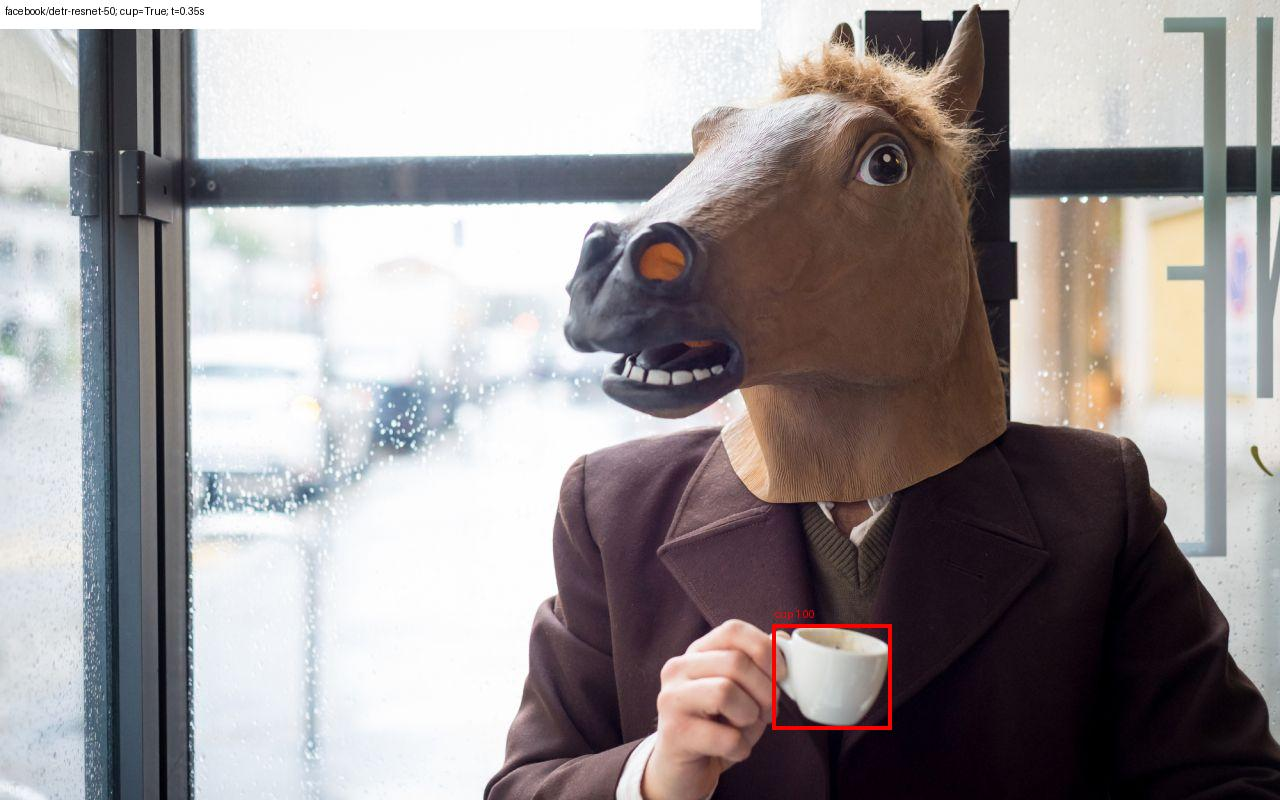
\includegraphics[width=\linewidth]{cup_detr.jpg}\caption{DETR}\end{subfigure}\hfill
\begin{subfigure}{0.32\textwidth}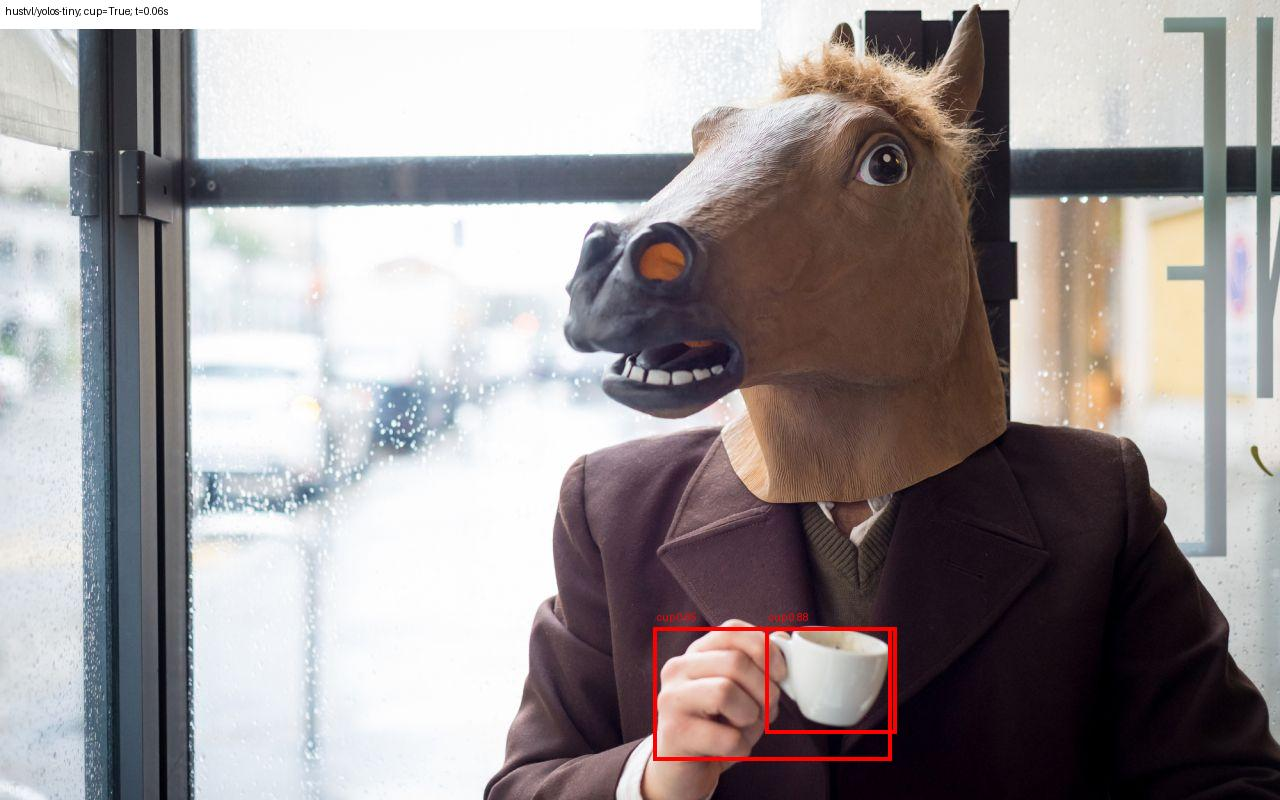
\includegraphics[width=\linewidth]{cup_yolos.jpg}\caption{YOLOS-tiny}\end{subfigure}\hfill
\begin{subfigure}{0.32\textwidth}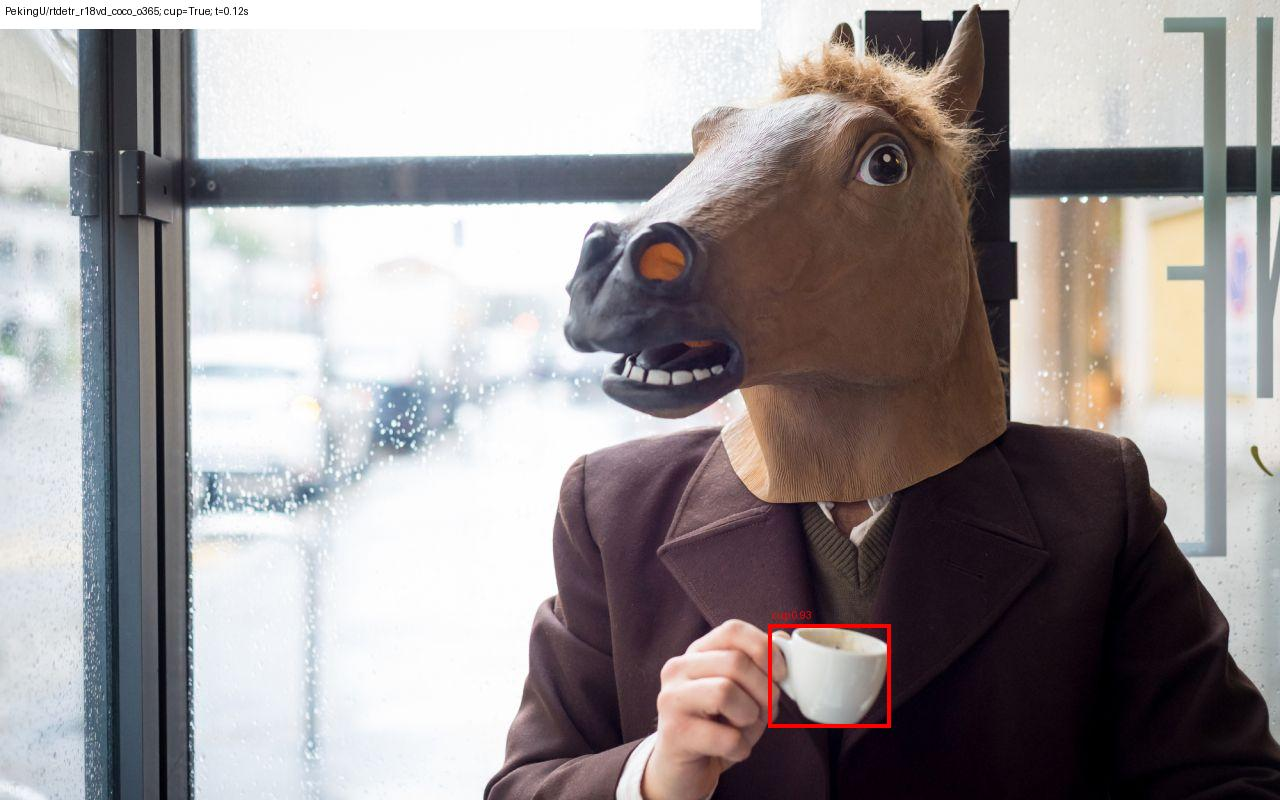
\includegraphics[width=\linewidth]{cup_rtdetr.jpg}\caption{RT-DETR}\end{subfigure}
\caption{Обнаружение маленькой чашки на изображении 4}\label{fig:cup-small}
\end{figure}

\begin{figure}[H]
\centering
\begin{subfigure}{0.32\textwidth}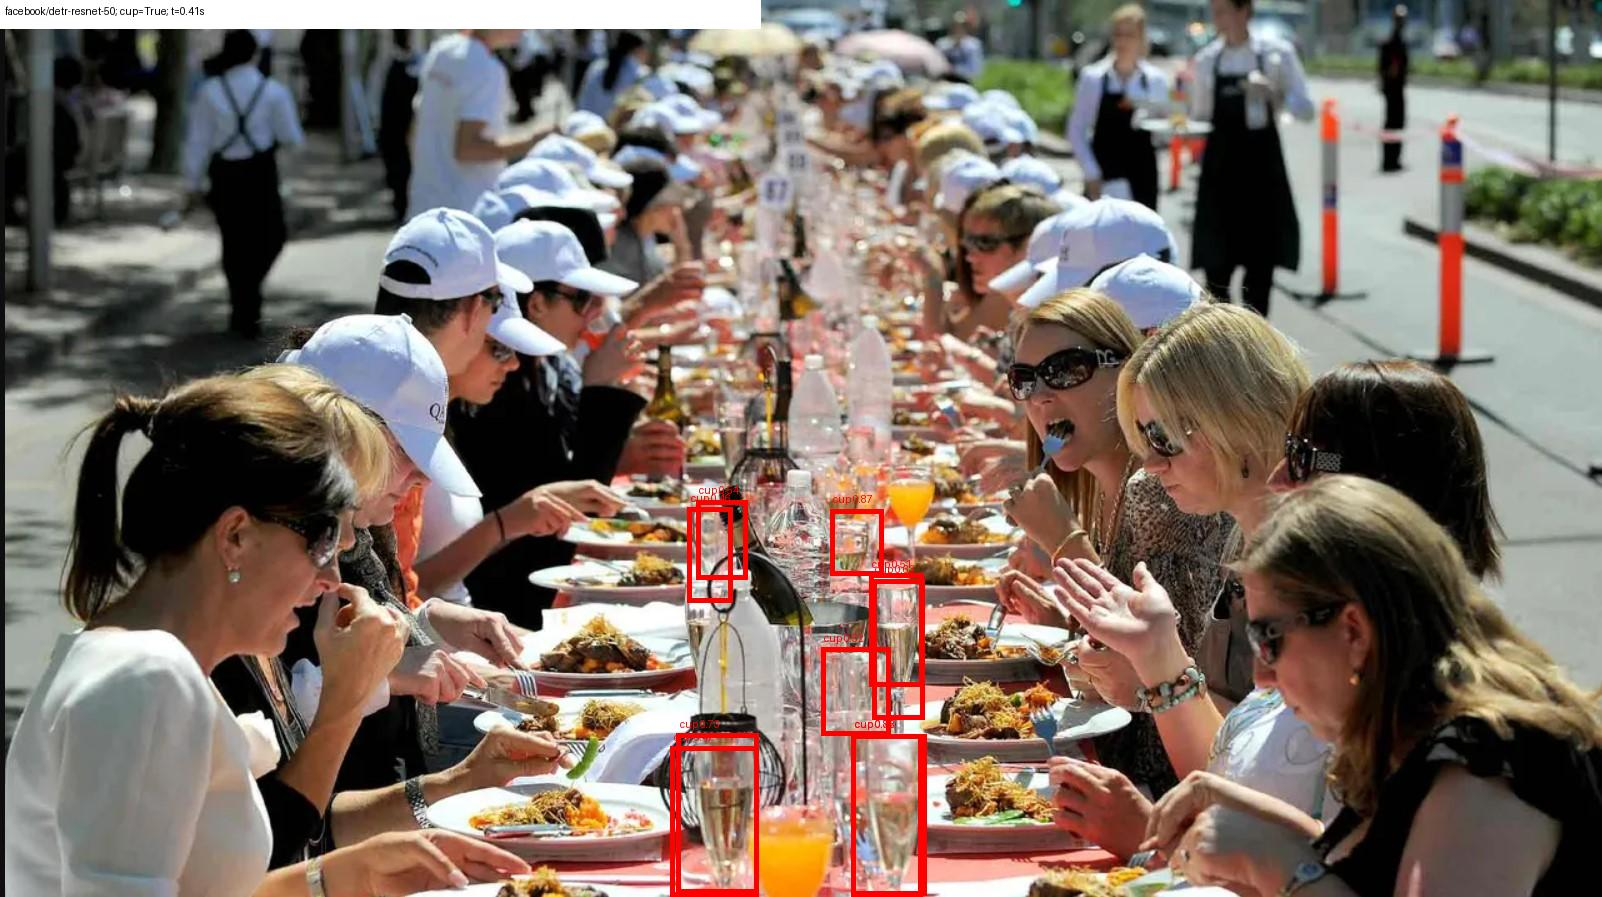
\includegraphics[width=\linewidth]{cup0_detr.jpg}\caption{DETR: 10 рамок}\end{subfigure}\hfill
\begin{subfigure}{0.32\textwidth}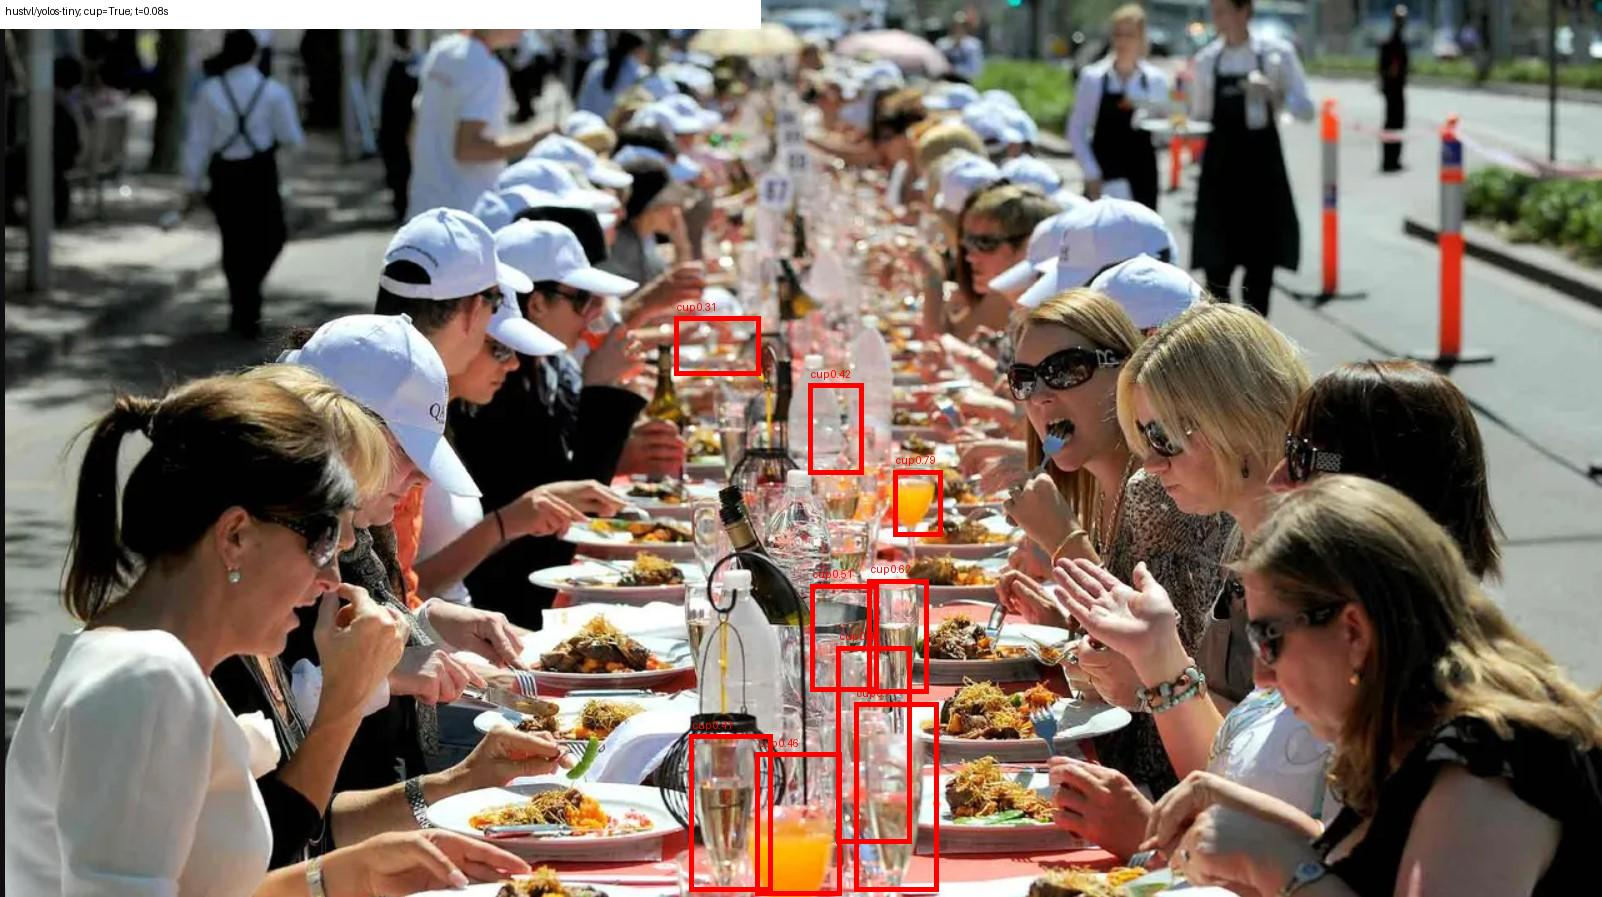
\includegraphics[width=\linewidth]{cup0_yolos.jpg}\caption{YOLOS: 9 рамок}\end{subfigure}\hfill
\begin{subfigure}{0.32\textwidth}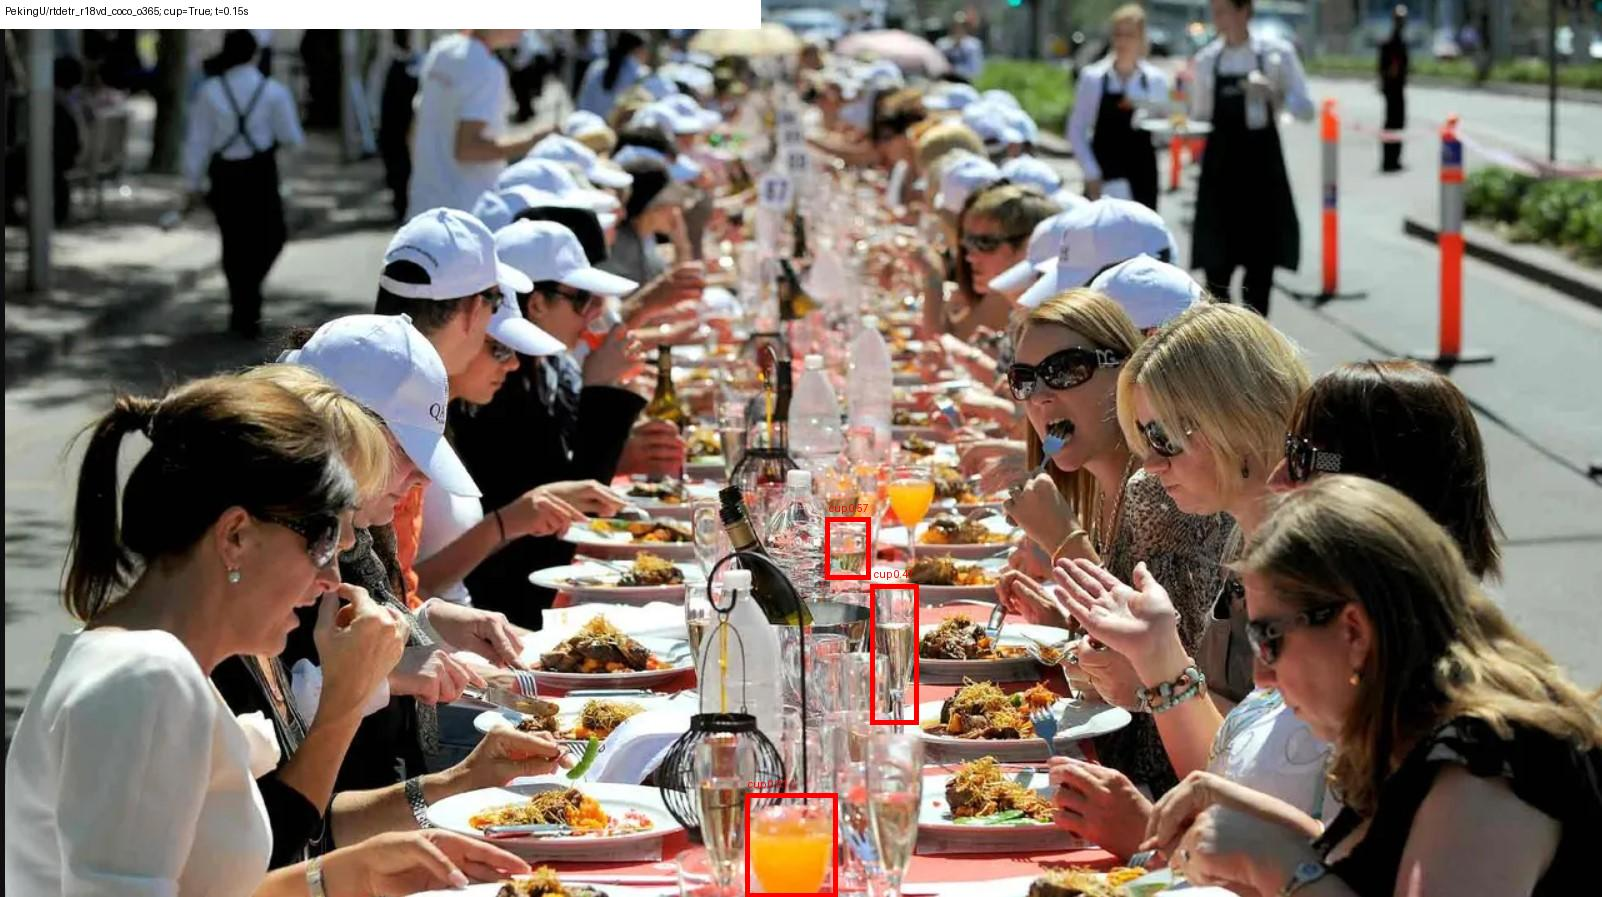
\includegraphics[width=\linewidth]{cup0_rtdetr.jpg}\caption{RT-DETR: 3 рамки}\end{subfigure}
\caption{Сложный отрицательный пример 0.jpg: модели обобщают класс cup на стеклянную посуду}\label{fig:cup-negative}
\end{figure}

\section{Проектные решения по обработке ошибок}

Основной источник ошибки --- не недостаток локализации, а неоднозначность таксономии. В бытовом русском языке бокал обычно не считается чашкой, тогда как датасет COCO объединяет в категории cup разнообразные сосуды для питья. Следовательно, срабатывания на \code{0.jpg} одновременно являются ложноположительными относительно строгой разметки работы и правдоподобными относительно исходного обучения. Для прикладной системы это исправляется уточнением требований, дополнительной классификацией crop-областей или дообучением на классах <<чашка>>, <<бокал>>, <<стакан>>.

DETR дополнительно ошибся на загруженном интерьере \code{5.jpg}. Возможные причины --- мелкие контрастные предметы на стойке и отсутствие NMS как отдельного фильтра. Повышение порога уменьшило бы число FP, но могло бы удалить слабое срабатывание YOLOS на \code{3.jpg}; поэтому порог следует выбирать на отдельной валидационной выборке, а не на пяти тестовых кадрах.

Ложноположительные рамки DETR на изображении 5 показаны на рисунке~\ref{fig:cup-fp}.

\begin{figure}[H]
\centering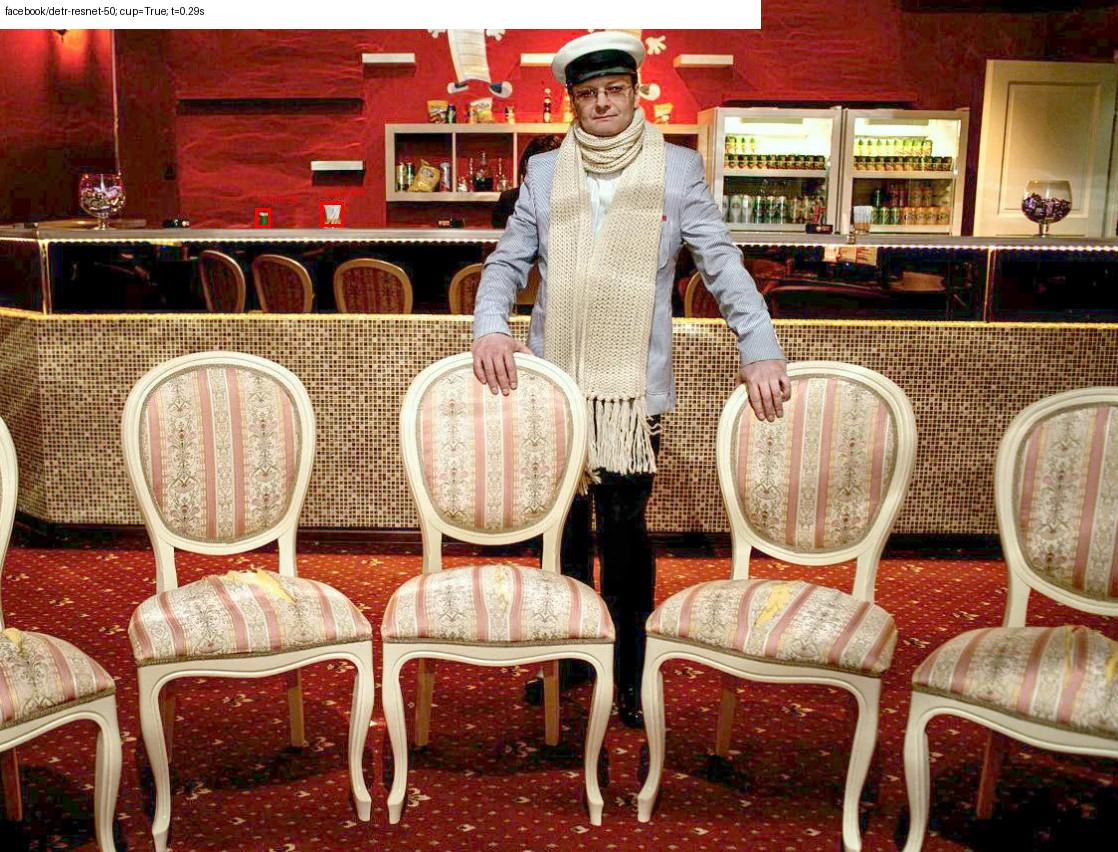
\includegraphics[width=0.72\textwidth]{cup_false_positive.jpg}
\caption{Ложноположительные рамки DETR на изображении 5}\label{fig:cup-fp}
\end{figure}

\section{Архитектура подсистемы параллельных прямых}

Модель сегментов не выдаёт готовый класс <<параллельные прямые>>, поэтому система проектируется как композиция двух независимых уровней. Первый уровень отвечает за зрительное восприятие и преобразует растровое изображение в множество отрезков $L=\{l_i\}$. Второй уровень является детерминированным: вычисляет углы, расстояния по нормали и формирует множество пар $P=\{(l_i,l_j)\}$.

Контракты программных подсистем приведены в таблице~\ref{tab:contracts}.

\begin{table}[H]
\centering\small
\caption{Контракты программных подсистем}
\label{tab:contracts}
\begin{tabularx}{\textwidth}{|>{\raggedright\arraybackslash}p{3cm}|>{\raggedright\arraybackslash}p{3.3cm}|>{\raggedright\arraybackslash}X|}
\hline
\multicolumn{1}{|c|}{Подсистема} & \multicolumn{1}{c|}{Вход и выход} & \multicolumn{1}{>{\centering\arraybackslash}X|}{Основные операции} \\
\hline
Детекция чашки & RGB-изображение $\rightarrow$ рамки, классы, уверенности & препроцессинг; forward; возврат координат; фильтр класса cup; визуализация\\ \hline
Детекция отрезков & RGB-изображение $\rightarrow$ координаты линий & resize $512\times512$; LiteRT-инференс; local maximum; декодирование; фильтр длины\\ \hline
Проверка параллельности & множество отрезков $\rightarrow$ пары & углы modulo $180^\circ$; циклическая разность; расстояние по нормали; ранжирование\\ \hline
Оценка & предсказания и разметка $\rightarrow$ JSON/CSV & матрица ошибок; метрики; время; RSS; формирование иллюстраций\\
\hline
\end{tabularx}
\end{table}

В обеих подсистемах вычислительное ядро отделено от ввода-вывода. Сценарий сначала формирует структурированную запись результата, затем на её основе рассчитывает метрики и строит изображение. Благодаря этому визуализация не влияет на измеряемое время инференса, а сохранённый JSON допускает повторный анализ без нового запуска модели.

\section{Алгоритмы программного комплекса}

\begingroup
Общий алгоритм исследования имеет следующий вид:
\begin{enumerate}
\item загрузить перечень файлов и заранее зафиксированную экспертную разметку;
\item загрузить процессор и веса модели, измерив время и изменение RSS;
\item выполнить инференс каждого изображения в режиме без вычисления градиентов;
\item применить специализированную постобработку: фильтр cup либо декодирование и сравнение отрезков;
\item сохранить детальные записи, аннотированные изображения и сводную таблицу;
\item вычислить метрики только после обработки всего набора;
\item освободить модель и сборщиком мусора вернуть неиспользуемые объекты перед загрузкой следующей.
\end{enumerate}

Отдельное проектное решение --- не зашивать числовой идентификатор класса cup. Название извлекается из \code{id2label}, поскольку разные конфигурации могут использовать различную нумерацию. Для линий аналогичным контрактом служит массив координат, не зависящий от того, какой детектор сформировал сегменты.
\endgroup

\Needspace{12\baselineskip}
\section{Выводы по конструкторскому разделу}

Спроектированы два конвейера: модель формирует первичные сущности, а детерминированная постобработка преобразует их в ответ задачи. Для обоих зафиксированы контракты входов и выходов, порядок измерения ресурсов и независимость от числовой нумерации классов.

Ключевые проектные решения состоят в следующем:
\begin{itemize}
\item подсистема поиска чашки использует единый интерфейс процессора и детектора, а класс выбирается по текстовой метке \code{cup}, поэтому модель можно заменить без изменения последующей обработки;
\item подсистема прямых отделяет нейросетевую детекцию отрезков от геометрической проверки углов и расстояний, что делает правило параллельности явным и проверяемым;
\item измерение загрузки, инференса и прироста RSS выполняется отдельно, поэтому опубликованные характеристики модели не смешиваются с результатами локального эксперимента;
\item JSON хранит исходные числовые результаты, CSV формирует сводку, а аннотированные изображения обеспечивают визуальную проверку ошибок.
\end{itemize}

Полученная архитектура допускает замену моделей, повторный пересчёт метрик без нового инференса и расширение тестовой выборки без изменения формата результатов.

\chapter{Технологическая часть}

В разделе описаны язык, библиотеки и программная реализация спроектированных конвейеров. Основным языком выбран Python 3.12: для него доступны официальные интерфейсы Hugging Face, PyTorch, LiteRT, NumPy и средства сохранения результатов в JSON/CSV. Исходные программы приведены полностью в приложениях~\ref{app:cups} и~\ref{app:lines}.

\section{Выбор языка, библиотек и форматов}

Использованные программные средства перечислены в таблице~\ref{tab:tools}.

\begin{table}[H]
\centering\small
\caption{Использованные программные средства}
\label{tab:tools}
\begin{tabularx}{\textwidth}{|>{\raggedright\arraybackslash}p{3.1cm}|>{\raggedright\arraybackslash}p{3.4cm}|>{\raggedright\arraybackslash}X|}
\hline
\multicolumn{1}{|c|}{Средство} & \multicolumn{1}{c|}{Назначение} & \multicolumn{1}{>{\centering\arraybackslash}X|}{Причина выбора} \\
\hline
Python 3.12 & управляющая логика & единая экосистема для всех выбранных моделей и анализа данных\\ \hline
PyTorch, Transformers & DETR, YOLOS, RT-DETR & официальные processor/model API и режим \code{inference_mode}\\ \hline
Hugging Face Hub & получение весов & кэширование и воспроизводимые идентификаторы репозиториев\\ \hline
LiteRT & M-LSD-tiny & компактный FP16-checkpoint и CPU-инференс без полной среды обучения\\ \hline
NumPy, SciPy & декодирование линий & векторные операции и фильтр локального максимума\\ \hline
Pillow & изображения & RGB-конвертация, рамки, линии и подписи\\ \hline
psutil & измерение ресурсов & получение RSS текущего процесса\\ \hline
JSON и CSV & результаты & JSON сохраняет детальные структуры, CSV удобен для табличного сравнения\\
\hline
\end{tabularx}
\end{table}

Программы не требуют графического интерфейса и запускаются из корня проекта. Пути формируются через \code{pathlib.Path}, каталоги результатов создаются автоматически, а текстовые файлы записываются в UTF-8. Такой подход одинаково работает в Windows и Unix-подобных системах при наличии зависимостей.

Команды запуска и состав электронного приложения приведены в приложении~\ref{app:repro}.

\section{Средства реализации и модели сегментов прямых}

Нейросетевые детекторы находят отдельные отрезки, а отношение параллельности определяется геометрическим постпроцессингом. Это делает решение интерпретируемым и позволяет явно задать допуск по углу.

Характеристики моделей сегментов прямых приведены в таблице~\ref{tab:line-models}.

\begin{table}[H]
\centering\small
\caption{Характеристики моделей сегментов прямых}
\label{tab:line-models}
\begin{tabularx}{\textwidth}{|>{\raggedright\arraybackslash}p{3.4cm}|>{\raggedright\arraybackslash}X|>{\raggedright\arraybackslash}p{3.2cm}|}
\hline
\multicolumn{1}{|c|}{Модель Hugging Face} & \multicolumn{1}{>{\centering\arraybackslash}X|}{Особенность} & \multicolumn{1}{c|}{Ресурсы} \\
\hline
\code{litert-community/M-LSD-tiny-LiteRT} & MobileNetV2 U-Net; карта центров и смещения концов; рассчитана на мобильные устройства & 0,62 млн параметров; FP16-файл 1,39 МБ; вход $512\times512$\\ \hline
\code{lh9171338/ULSD} & единое представление прямых и искажённых сегментов кривой Безье; варианты для pinhole, fisheye и spherical & pinhole 40,4 МБ; mixed 160,9 МБ; PyTorch 1.6, CUDA 10.1 в исходной реализации\\ \hline
\code{cherubicxn/scalelsd} & ViT-base и масштабируемое самоконтролируемое обучение на SA-1B; v2 использует LayerScale и AdamW & v2 493,5 МБ; Python 3.10, PyTorch 2.5.1, CUDA 12.1 в эталонной среде\\
\hline
\end{tabularx}
\end{table}

Для M-LSD-tiny при $512\times512$ в статье приведены $F^H=77{,}2$, $sAP^{10}=58{,}0$ на Wireframe, 0,6 млн параметров и 164,1 кадра/с на Tesla V100. На Raspberry Pi 5 карточка LiteRT приводит медиану 106,6 мс и пиковую память 75 МБ. Для ULSD на Wireframe приведены $sAP^{10}=69{,}2$, $F^H=80{,}4$ и 37,2 кадра/с для одного из вариантов. У ScaleLSD карточка весов не содержит числовой таблицы метрик, а рекомендуемый v2 отличается от версии, оценённой в исходной статье; поэтому неподтверждённое число в отчёт не включалось.

\subsection{M-LSD-tiny}

M-LSD~\cite{gu} --- облегчённый детектор отрезков на основе MobileNetV2 и U-Net-подобного декодера. Вместо перебора всех пар граничных пикселей сеть предсказывает карту центров и геометрические смещения от центра к двум концам. Дополнительные признаки segment of line (SoL) и matching помогают обучить модель при небольшом числе параметров. Выход затем декодируется в явные координаты отрезков.

Выбранный репозиторий содержит конвертацию в LiteRT. Модель подходит для мобильных и CPU-сценариев: FP16-файл занимает 1,39 МБ, а карточка сообщает 75 МБ пиковой памяти на Raspberry Pi 5. Ограничение облегчённой архитектуры --- множество коротких либо дублирующихся сегментов на текстурированных схемах, поэтому постобработка обязательна.

\subsection{ULSD}

ULSD~\cite{li} решает более широкий класс задач: отрезки на pinhole-изображениях и кривые линии после fisheye/spherical-проекции представлены единообразно параметрической кривой Безье. Сеть предсказывает centre, endpoints и управляющие точки, после чего специальный модуль восстанавливает геометрию. Поэтому ULSD целесообразен для панорамных камер, где физически прямой объект становится кривой на изображении.

Репозиторий Hugging Face хранит несколько checkpoint: pinhole, fisheye, spherical и mixed. Это повышает гибкость, но усложняет развёртывание: исходная реализация привязана к PyTorch 1.6 и CUDA 10.1, а каждый специализированный файл около 40,4 МБ. Для современной среды может понадобиться адаптация зависимостей и пользовательского декодера.

\subsection{ScaleLSD v2}

ScaleLSD~\cite{ke} использует ViT-признаки и масштабируемое самоконтролируемое обучение на автоматически сформированных данных SA-1B. Цель --- перенос на новые домены без разметки: архитектурные сцены, дороги, рисунки и изображения, отличающиеся от Wireframe. Карточка рекомендует v2 с LayerScale и AdamW и прямо отмечает, что эта версия работает существенно лучше ранней конфигурации статьи.

Цена универсальности --- самый тяжёлый checkpoint: около 493,5 МБ, то есть примерно в 355 раз больше FP16-весов M-LSD-tiny. Эталонная среда использует Python 3.10, PyTorch 2.5.1 и CUDA 12.1; для комфортного исследования практически необходима современная GPU.

\section{Требования к программной и аппаратной среде}

Опубликованные результаты детекторов линий приведены в таблице~\ref{tab:line-published}.

\begin{table}[H]
\centering\small
\caption{Опубликованные результаты детекторов линий}
\label{tab:line-published}
\begin{tabularx}{\textwidth}{|l|r|r|r|r|X|}
\hline
\multicolumn{1}{|c|}{Модель} & \multicolumn{1}{c|}{$sAP^{10}$} & \multicolumn{1}{c|}{$F^H$} & \multicolumn{1}{c|}{Скорость} & \multicolumn{1}{c|}{Набор} & \multicolumn{1}{>{\centering\arraybackslash}X|}{Комментарий} \\
\hline
M-LSD-tiny & 58,0 & 77,2 & 164,1 FPS & Wireframe & $512\times512$, Tesla V100\\ \hline
ULSD & 69,2 & 80,4 & 37,2 FPS & Wireframe & один из pinhole-вариантов\\ \hline
ScaleLSD & --- & --- & --- & SA-1B transfer & v2 отличается от оценённой в статье v1\\
\hline
\end{tabularx}
\end{table}

$sAP^{10}$ требует близости предсказанных и истинных концов, а $F^H$ измеряет совпадение пикселей/линий. Эти метрики характеризуют качество отдельных сегментов, но не готовность ответа <<есть параллельная пара>>. Нельзя утверждать, что 69,2 означает 69,2~\% точности поиска параллельных прямых: геометрическое отношение возникает только на следующем этапе.

В статье ScaleLSD для zero-shot переноса с SA-1B приведена Repeatability-5 0,725 на YorkUrban и 0,367 на HPatches, а для vanishing point estimation на YUD+ --- ошибка около 1,55 и AUC 87,1. Эти показатели относятся к другим протоколам и потому не включены в одну числовую колонку с Wireframe $sAP$.

Требования к ресурсам и развёртыванию моделей линий сведены в таблице~\ref{tab:line-requirements}.

\begin{table}[H]
\centering\small
\caption{Требования к ресурсам и развёртыванию моделей линий}
\label{tab:line-requirements}
\begin{tabularx}{\textwidth}{|>{\raggedright\arraybackslash}p{2.7cm}|r|r|>{\raggedright\arraybackslash}X|}
\hline
\multicolumn{1}{|c|}{Модель} & \multicolumn{1}{c|}{Параметры/веса} & \multicolumn{1}{c|}{Память/среда} & \multicolumn{1}{>{\centering\arraybackslash}X|}{Практическая оценка} \\
\hline
M-LSD-tiny & 0,62 млн; 1,39 МБ FP16 & 75 МБ peak на RPi 5 & пригодна для CPU, edge и мобильных устройств\\ \hline
ULSD & около 40,4 МБ на checkpoint & PyTorch 1.6, CUDA 10.1 & нужна совместимая среда либо перенос кода\\ \hline
ScaleLSD v2 & 493,5 МБ & PyTorch 2.5.1, CUDA 12.1 & исследовательский GPU-сценарий\\
\hline
\end{tabularx}
\end{table}

\section{Реализация M-LSD и геометрической постобработки}

Изображение приводилось к $512\times512$, добавлялся четвёртый канал единиц, значения масштабировались в диапазон $[-1,1]$. Сеть возвращала карту $9\times256\times256$. После сигмоиды, локального максимума $3\times3$ и порога 0,10 декодировались до 200 отрезков длиной более 20 пикселей. Затем попарно сравнивались их углы.

Последовательность обработки состоит из пяти этапов:

\begin{enumerate}
\item сохранить исходное соотношение сторон для последующего возврата координат;
\item привести изображение к входу $512\times512$ и выполнить нормализацию LiteRT;
\item декодировать локальные максимумы карты центров и смещения концов;
\item удалить слишком короткие сегменты, вычислить направление каждого оставшегося;
\item перебрать пары, применить угловой и пространственный критерии, визуализировать результат.
\end{enumerate}

\begin{lstlisting}
delta = abs(alpha_i - alpha_j) % 180.0
delta = min(delta, 180.0 - delta)
parallel = delta <= 3.0 and normal_distance >= 4.0
\end{lstlisting}

Проверка расстояния по нормали исключает сравнение практически одного и того же отрезка с его дубликатом. Однако она не устраняет все комбинааторные повторы. Для производственной версии следует сначала кластеризовать направления, затем объединять коллинеарные фрагменты и выбирать репрезентативные пары с достаточной длиной и перекрытием проекций.

\section{Формирование и сохранение результатов}

Результаты M-LSD-tiny на изображениях преподавателя приведены в таблице~\ref{tab:line-run}.

\begin{table}[H]
\centering
\caption{M-LSD-tiny на изображениях преподавателя}
\label{tab:line-run}
\begin{tabular}{|l|r|r|r|}
\hline
\multicolumn{1}{|c|}{Файл} & \multicolumn{1}{c|}{Отрезки} & \multicolumn{1}{c|}{Пары параллельных} & \multicolumn{1}{c|}{Время, с} \\
\hline
6.png & 97 & 1495 & 0,098\\ \hline
7.png & 112 & 1828 & 0,099\\ \hline
8.png & 194 & 6617 & 0,100\\ \hline
9.jpg & 65 & 118 & 0,098\\ \hline
10.jpg & 124 & 522 & 0,101\\ \hline
11.jpg & 101 & 570 & 0,100\\
\hline
\end{tabular}
\end{table}

Параллельные пары найдены на всех 6 из 6 положительных изображений, то есть полнота по изображениям равна 1,00. Среднее время инференса составило 0,099 с, загрузка локального LiteRT-файла --- 0,028 с, прирост RSS --- около 51,4 МБ. Большое число пар на схемах ожидаемо: множество сторон прямоугольников имеют одинаковое направление, и каждая комбинация считается отдельно.

Примеры найденных отрезков и параллельных пар приведены на рисунке~\ref{fig:lines}.

\begin{figure}[H]
\centering
\begin{subfigure}{0.48\textwidth}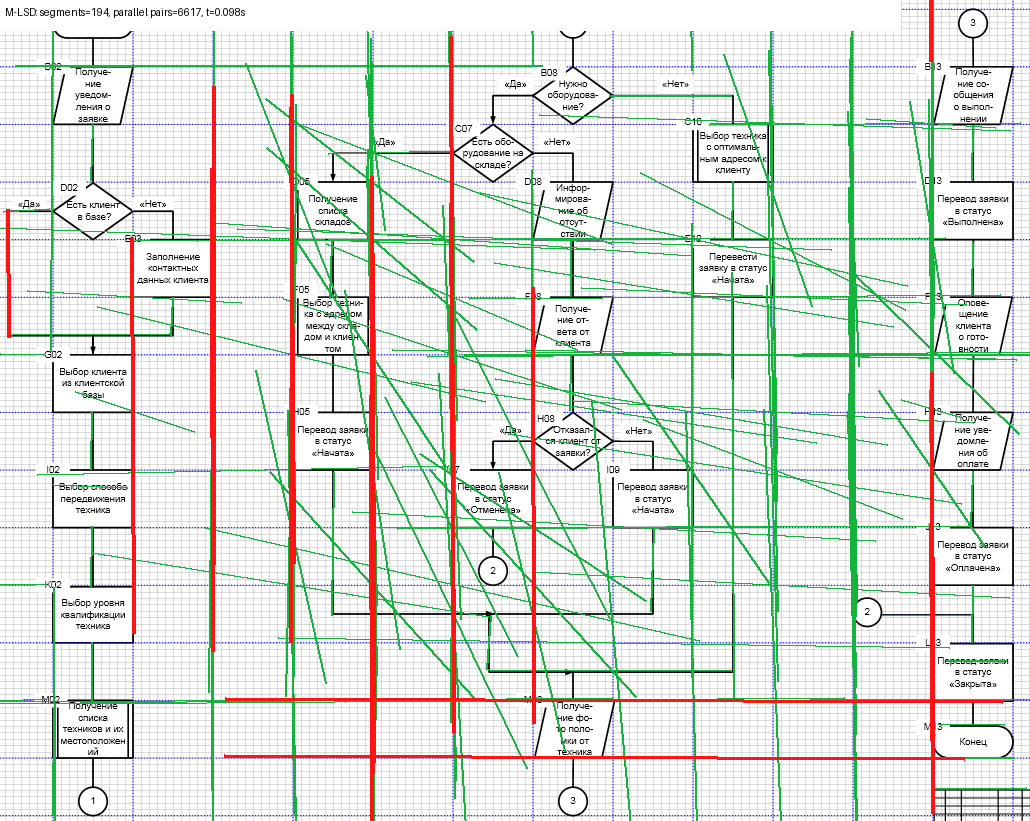
\includegraphics[width=\linewidth]{lines_scheme.png}\caption{Блок-схема}\end{subfigure}\hfill
\begin{subfigure}{0.48\textwidth}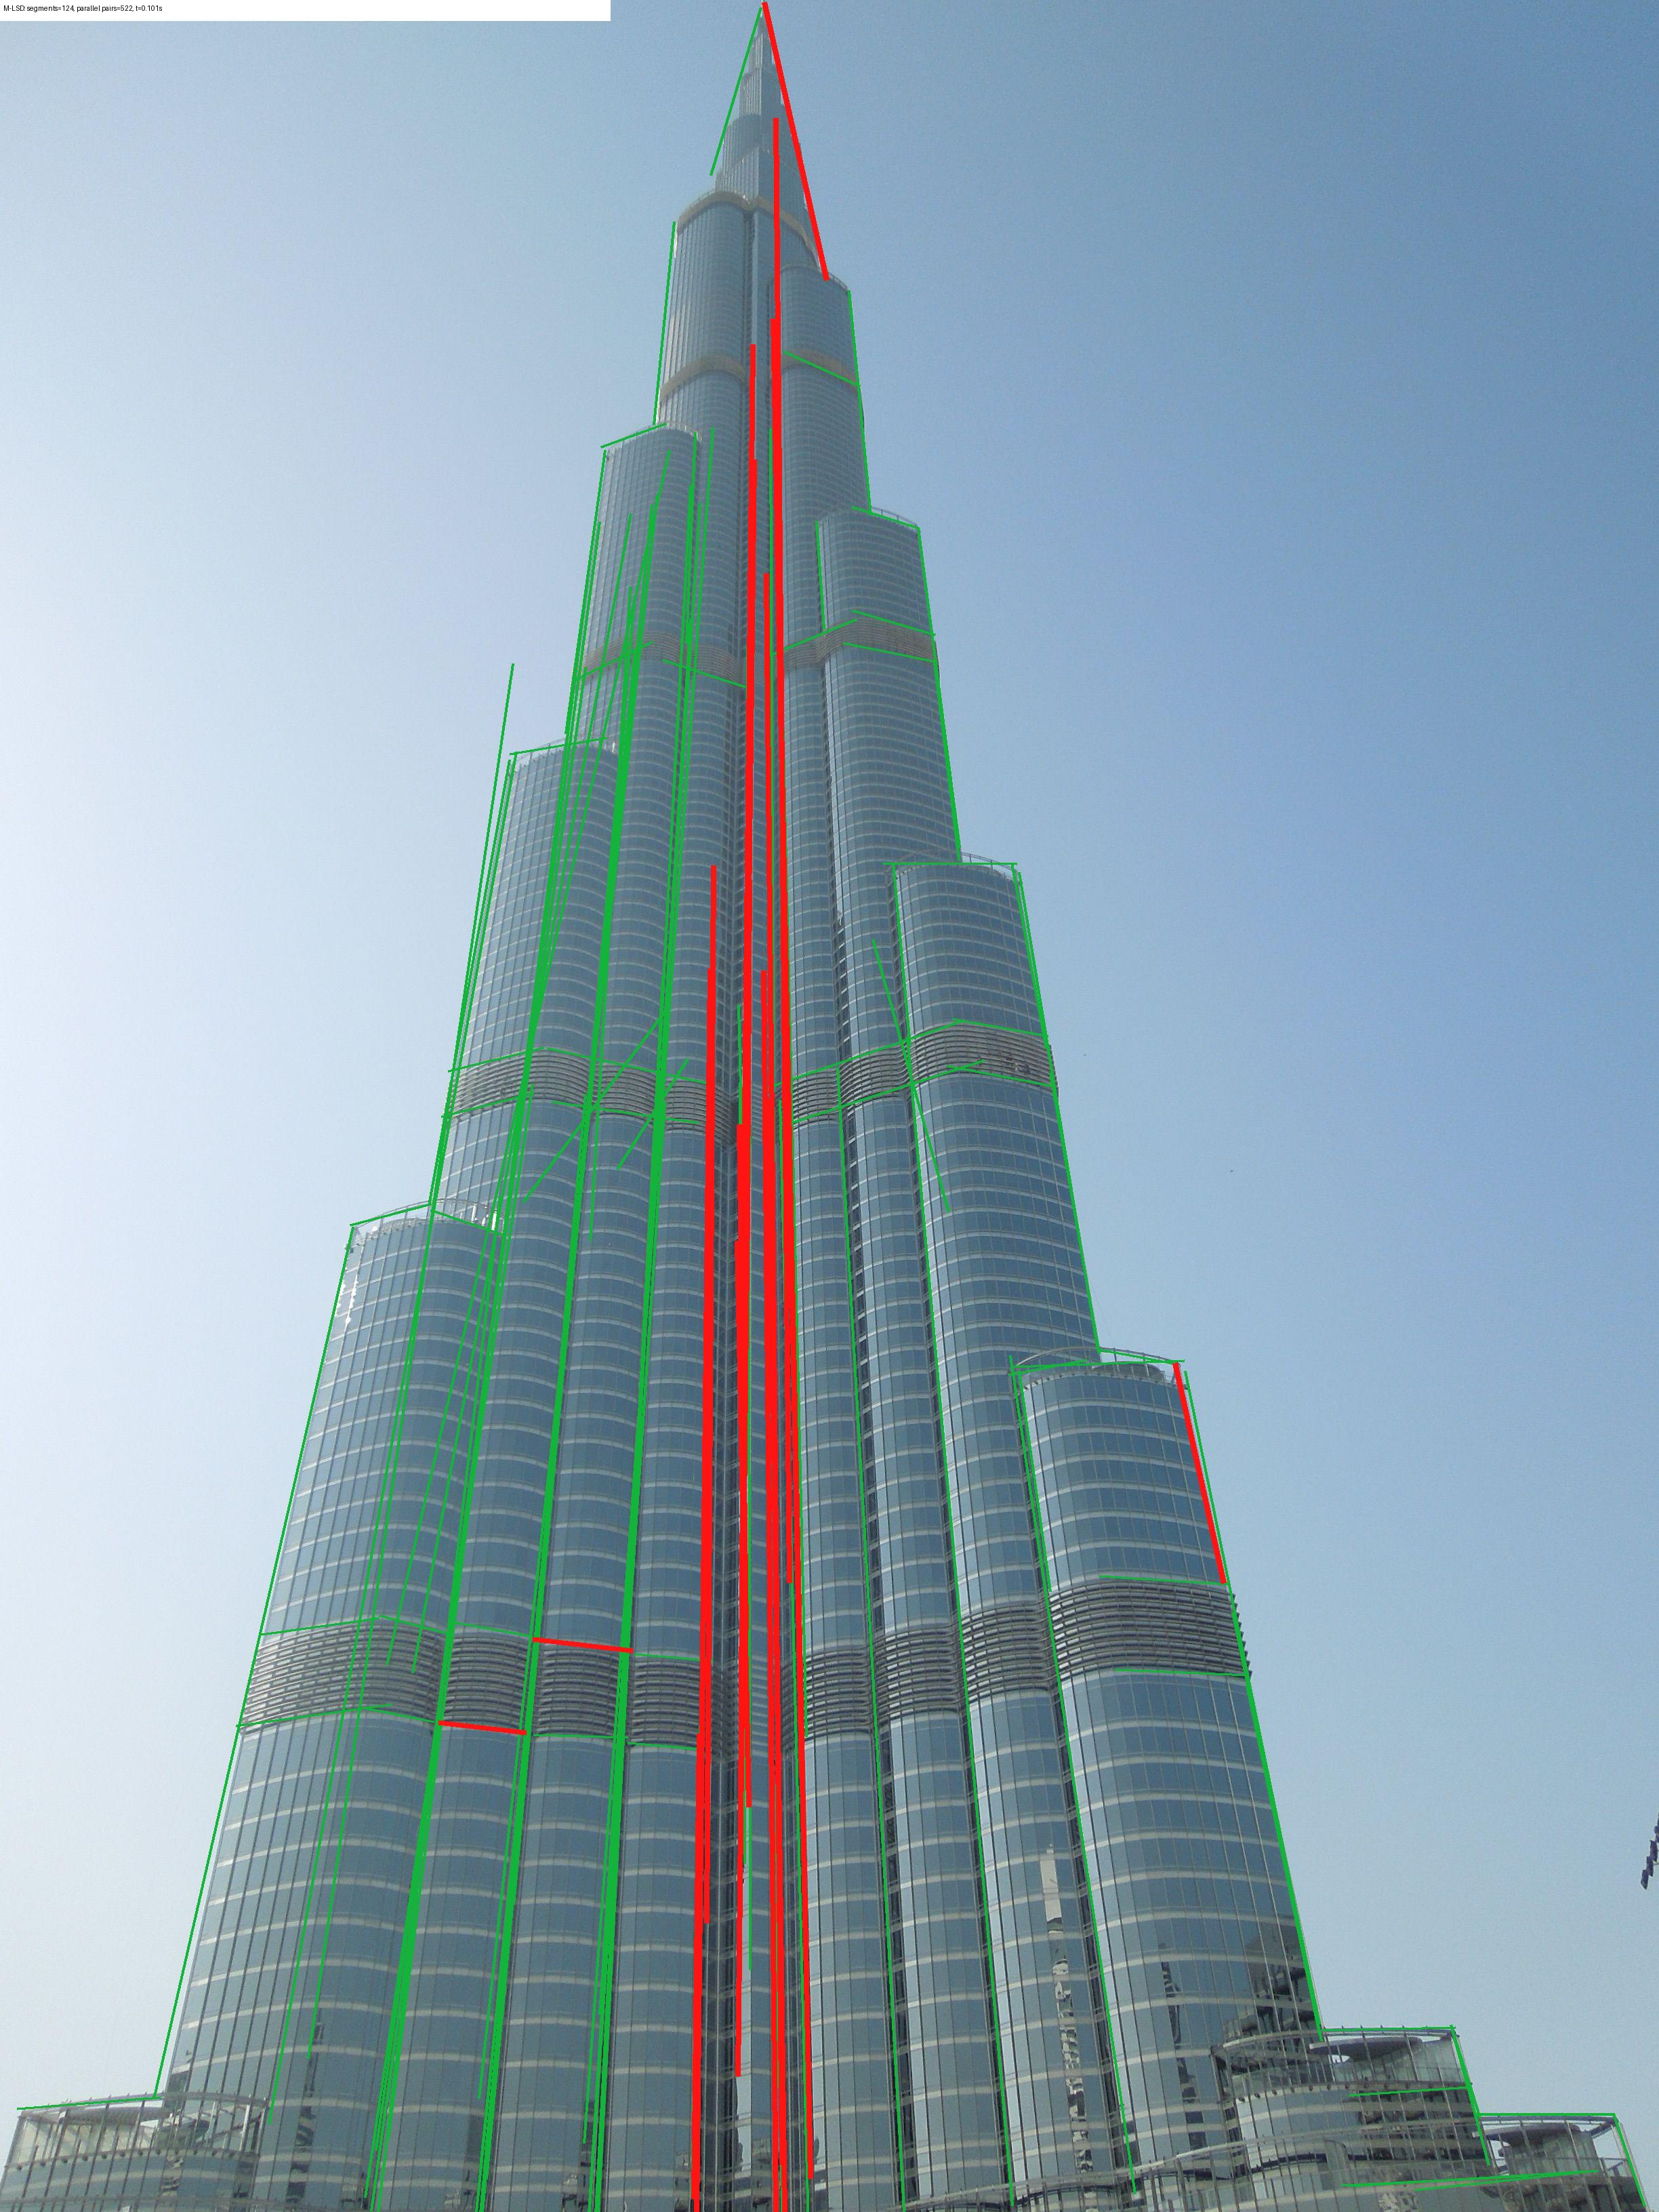
\includegraphics[width=\linewidth]{lines_building.jpg}\caption{Фасад здания}\end{subfigure}
\caption{Результаты M-LSD: зелёные линии --- найденные отрезки, красные --- представители параллельных пар}\label{fig:lines}
\end{figure}

\section{Обработка ограничений и вырожденных случаев}

Полученная полнота 1,00 означает лишь, что на каждом положительном кадре существует хотя бы одна найденная пара. Она ничего не говорит о числе ложных пар: отрицательных изображений без параллельных прямых в предоставленном поднаборе нет. Кроме того, при перспективной съёмке параллельные в трёхмерном мире рёбра сходятся к точке исчезновения и перестают быть параллельными в координатах изображения. Угловой допуск $3^\circ$ работает для слабой перспективы, но для фасада, снятого снизу, корректнее оценивать общую vanishing point.

Схемы создают другую проблему: M-LSD выделяет рамки блоков, стрелки, символы и сетку как множество коротких линий, после чего число пар растёт квадратично. Практическое решение должно ранжировать пары по длине, сходству направления и пространственной связности, а не возвращать тысячи равноправных комбинаций.

\Needspace{12\baselineskip}
\section{Выводы по технологической части}

Реализация выполнена на Python 3.12 с использованием PyTorch/Transformers для объектной детекции и LiteRT для M-LSD. Программы автоматически создают каталоги, измеряют время и RSS, сохраняют подробный JSON, сводный CSV и аннотированные изображения. Полные исходные тексты вынесены в приложения А и Б, что позволяет воспроизвести все приведённые локальные показатели.

В ходе реализации обеспечены следующие свойства:
\begin{itemize}
\item единый цикл запуска трёх моделей чашки на одной размеченной выборке и при одном пороге уверенности;
\item отдельный LiteRT-конвейер декодирования M-LSD с возвратом координат в исходное разрешение;
\item сохранение времени загрузки, среднего времени инференса и изменения RSS раздельными полями;
\item автоматическое формирование таблиц и иллюстраций из тех же структурированных результатов, которые используются при расчёте метрик.
\end{itemize}

Ограничения реализации также зафиксированы явно: бинарная оценка чашки не заменяет IoU/AP, а положительная выборка прямых не позволяет измерить специфичность и число ложных пар.

\chapter{Исследовательский раздел}

\section{Объекты исследования и методика оценки}

Исследуются две группы решений. В первой группе три COCO-детектора обрабатывают одинаковые пять изображений при едином пороге 0,30. Экспертная разметка фиксируется до запуска: \code{3.jpg} и \code{4.jpg} положительные, остальные отрицательные. Сравниваются TP, TN, FP, FN, Accuracy, Precision, Recall, $F_1$, среднее CPU-время и прирост RSS.

Во второй группе сопоставляются три подхода к обнаружению сегментов по официальным метрикам и ресурсам, а M-LSD-tiny дополнительно запускается на шести изображениях. Для локального опыта проверяется наличие хотя бы одной пары с разностью направлений не более $3^\circ$ и нормальным расстоянием не менее 4 пикселей. Поскольку отрицательных кадров нет, вычисляется только полнота по положительным изображениям; значение не интерпретируется как precision.

Чтобы не смешивать независимые шкалы, опубликованные COCO AP, Wireframe $sAP$, $F^H$, repeatability и AUC рассматриваются отдельно от локальной бинарной оценки. Время загрузки весов, время инференса и визуализация также разделены. Такой протокол позволяет проследить происхождение каждого численного вывода.

\section{Результаты исследования обнаружения чашки}

Итоговое сравнение моделей обнаружения чашки приведено в таблице~\ref{tab:cup-final}.

\begin{table}[H]
\centering\small
\caption{Итоговое сравнение моделей обнаружения чашки}
\label{tab:cup-final}
\begin{tabular}{|l|r|r|r|r|r|}
\hline
\multicolumn{1}{|c|}{Модель} & \multicolumn{1}{c|}{Accuracy} & \multicolumn{1}{c|}{Precision} & \multicolumn{1}{c|}{Recall} & \multicolumn{1}{c|}{$F_1$} & \multicolumn{1}{c|}{CPU, с/кадр} \\
\hline
DETR ResNet-50 & 0,60 & 0,50 & 1,00 & 0,67 & 0,353\\ \hline
YOLOS-tiny & 0,80 & 0,67 & 1,00 & 0,80 & 0,065\\ \hline
RT-DETR-R18 & 0,80 & 0,67 & 1,00 & 0,80 & 0,120\\
\hline
\end{tabular}
\end{table}

Все три модели нашли обе явные чашки, поэтому Recall равен 1,00. Различие возникло на отрицательных сценах. Каждый детектор отнёс часть стеклянной посуды в \code{0.jpg} к cup; DETR дополнительно сформировал ложный положительный ответ на \code{5.jpg}. Поэтому лучшие локальные $F_1=0,80$ получили YOLOS-tiny и RT-DETR.

Результат нельзя сводить только к локальной Accuracy. YOLOS минимизирует ресурсы и показал 0,065 с/кадр при приросте RSS 25,7 МБ. RT-DETR медленнее, но имеет наиболее высокий опубликованный COCO AP 49,2. Следовательно, выбор зависит от приоритета: YOLOS для ограниченного CPU, RT-DETR для более высокого ожидаемого качества на разнообразных сценах.

\section{Результаты исследования параллельных прямых}

Итог локального запуска M-LSD-tiny приведён в таблице~\ref{tab:lines-final}.

\begin{table}[H]
\centering\small
\caption{Итог локального запуска M-LSD-tiny}
\label{tab:lines-final}
\begin{tabular}{|l|r|r|r|r|}
\hline
\multicolumn{1}{|c|}{Изображений} & \multicolumn{1}{c|}{С найденной парой} & \multicolumn{1}{c|}{Полнота} & \multicolumn{1}{c|}{Среднее время, с} & \multicolumn{1}{c|}{Прирост RSS, МБ} \\
\hline
6 & 6 & 1,00 & 0,099 & 51,4\\
\hline
\end{tabular}
\end{table}

Положительный результат на всех шести файлах подтверждает работоспособность конвейера, но число сформированных пар --- от 118 до 6617 --- показывает недостаточность простого попарного перебора для пользовательского вывода. На схемах повторяются стороны блоков и линии сетки; на зданиях перспектива изменяет углы. Следовательно, после детекции необходимы кластеризация направлений, объединение коллинеарных отрезков и ранжирование пар.

Из трёх моделей именно M-LSD-tiny практически проверена локально и имеет минимальные ресурсы. ULSD обоснован для fisheye/spherical-проекций, а ScaleLSD --- для тяжёлого zero-shot исследования с GPU. Эти рекомендации основаны на разных типах свидетельств и потому в таблицах явно разделены измеренные и опубликованные показатели.

\section{Матрица выбора}

Рекомендуемый выбор в зависимости от условий приведён в таблице~\ref{tab:choice}.

\begin{table}[H]
\centering\small
\caption{Рекомендуемый выбор в зависимости от условий}
\label{tab:choice}
\begin{tabularx}{\textwidth}{|>{\raggedright\arraybackslash}p{3.6cm}|>{\raggedright\arraybackslash}p{3.3cm}|>{\raggedright\arraybackslash}X|}
\hline
\multicolumn{1}{|c|}{Условие} & \multicolumn{1}{c|}{Рекомендуемая модель} & \multicolumn{1}{>{\centering\arraybackslash}X|}{Обоснование} \\
\hline
максимальное качество чашки из трёх & RT-DETR-R18 & максимальный COCO AP 49,2; локально Accuracy 0,80 и Recall 1,00\\ \hline
минимальные CPU-ресурсы & YOLOS-tiny & 26 МБ весов, 0,065 с/кадр, прирост RSS 25,7 МБ\\ \hline
базовая воспроизводимая архитектура & DETR ResNet-50 & простой end-to-end принцип без NMS, но наибольшие локальные затраты\\ \hline
edge-поиск прямых & M-LSD-tiny & 1,39 МБ FP16, быстрый LiteRT, полный локальный прогон\\ \hline
fisheye или панорамы & ULSD & единая кривая Безье для разных проекций\\ \hline
zero-shot перенос линий & ScaleLSD v2 & обучение на SA-1B и ViT-признаки, но тяжёлые веса\\
\hline
\end{tabularx}
\end{table}

Для обнаружения чашки рекомендуется RT-DETR-R18: он сохранил полноту 1,00, показал 0,80 правильных бинарных решений на пользовательском наборе и имеет наибольший опубликованный COCO AP среди трёх выбранных моделей. Если важны минимальный размер и скорость CPU, предпочтителен YOLOS-tiny: он в 3,1 раза меньше RT-DETR по числу параметров и в локальном тесте оказался примерно вдвое быстрее.

Для поиска параллельных прямых практическим выбором является M-LSD-tiny с геометрическим постпроцессингом. Модель компактна, запускается без дискретной GPU и успешно обработала все выданные изображения. ULSD целесообразен, если имеются сильные перспективные или оптические искажения. ScaleLSD подходит для более тяжёлой исследовательской системы с современной GPU, но его файл весов примерно в 355 раз больше FP16-файла M-LSD-tiny.

\section{Угрозы достоверности}

\begin{enumerate}
\item \emph{Малый набор.} Пять изображений чашек и шесть изображений линий позволяют продемонстрировать конвейер, но не дают узких доверительных интервалов и не охватывают все условия съёмки;
\item \emph{Неоднозначная разметка.} Стеклянная посуда в \code{0.jpg} может интерпретироваться как класс COCO cup. В отчёте заранее зафиксировано строгое бытовое определение чашки, чтобы не менять истину после получения результата;
\item \emph{Разные опубликованные протоколы.} COCO AP, Wireframe $sAP$, repeatability и AUC нельзя складывать или непосредственно ранжировать. Они приведены только в своих контекстах;
\item \emph{Не все тяжёлые модели запущены локально.} Для ULSD и ScaleLSD приведены официальные характеристики и анализ интеграции; эмпирически на изображениях преподавателя выполнен M-LSD. Это явно отделено от измеренных результатов;
\item \emph{Аппаратная зависимость.} Время CPU, RSS, GPU FPS и Raspberry Pi latency получены на разных платформах. Их следует использовать как ориентиры класса ресурсов, а не как прямой benchmark.
\end{enumerate}

\section{Как повысить качество исследования}

Следующий корректный эксперимент должен включать не менее 50--100 изображений на задачу, отдельные train/validation/test части, отрицательные кадры для линий и ручную разметку рамок/отрезков. Для чашек следует построить precision--recall кривую по нескольким порогам и рассчитать $AP_{50}$. Для линий --- сопоставить сегменты по расстоянию концов, посчитать precision/recall пар и отдельно оценить vanishing-point подход на архитектурных фотографиях. Повторение каждого замера времени после прогрева позволит привести медиану и квантили вместо одного среднего.

\section{Выводы по исследовательскому разделу}

На локальной выборке лучшую совокупность бинарных метрик показали YOLOS-tiny и RT-DETR-R18, однако модель выбирается с учётом разных целей: YOLOS минимизирует CPU-затраты, RT-DETR имеет наиболее высокий опубликованный COCO AP. M-LSD-tiny обнаружила параллельные пары на всех положительных изображениях и пригодна для CPU, но нуждается в сокращении комбинаторного числа пар. Результаты ограничены размером и составом набора и не объявляются универсальным рейтингом моделей.

\structel{ЗАКЛЮЧЕНИЕ}

На Hugging Face выбраны шесть уникальных моделей: DETR ResNet-50, YOLOS-tiny и RT-DETR-R18 для чашек; M-LSD-tiny, ULSD и ScaleLSD v2 для сегментов прямых. Ни одна из них не входит в список восьми уже занятых моделей, поэтому совпадение равно 0~\% и условие не более 34~\% выполнено.

Исследование не ограничилось описанием карточек. Для каждой модели разобраны архитектура, формат выхода, программная интеграция, опубликованные метрики и ресурсы. Три модели чашек воспроизводимо протестированы на пяти изображениях. Все нашли обе явные чашки; DETR получил Accuracy 0,60 и $F_1=0,67$, YOLOS-tiny и RT-DETR --- Accuracy 0,80 и $F_1=0,80$. YOLOS был самым лёгким локально, а RT-DETR сочетал локальный результат с максимальным COCO AP 49,2.

Для параллельных прямых реализован двухступенчатый конвейер M-LSD-tiny плюс геометрическая проверка углов. Пары найдены на всех шести положительных изображениях при среднем времени 0,099 с на CPU и приросте RSS 51,4 МБ. Этот результат подтверждает работоспособность, но не измеряет precision из-за отсутствия отрицательных кадров и разметки всех истинных пар. Практический итог работы состоит в том, что поиск объекта и поиск геометрического отношения требуют разных архитектур, разных постпроцессоров и разных протоколов оценки.

Таким образом, поставленная цель достигнута. Определён и проверен уникальный набор моделей; изучены их архитектуры и опубликованные показатели; спроектированы и реализованы два программных конвейера; выполнен воспроизводимый запуск на изображениях преподавателя; измерены качество и ресурсы; сформулированы рекомендации и ограничения. Все задачи, перечисленные во введении, выполнены.

\begin{thebibliography}{99}
\bibitem{omdet} Hugging Face. omlab/omdet-turbo-swin-tiny-hf : карточка модели, учтена как занятая.~--- URL: \url{https://huggingface.co/omlab/omdet-turbo-swin-tiny-hf} (дата обращения: 05.11.2026).
\bibitem{yoloe} Hugging Face. openvision/yoloe26-s-seg : карточка модели, учтена как занятая.~--- URL: \url{https://huggingface.co/openvision/yoloe26-s-seg} (дата обращения: 05.11.2026).
\bibitem{clipseg} Hugging Face. CIDAS/clipseg-rd64-refined : карточка модели, учтена как занятая.~--- URL: \url{https://huggingface.co/CIDAS/clipseg-rd64-refined} (дата обращения: 05.11.2026).
\bibitem{hf-detr} Hugging Face. facebook/detr-resnet-50 : карточка модели.~--- URL: \url{https://huggingface.co/facebook/detr-resnet-50} (дата обращения: 05.11.2026).
\bibitem{hf-yolos} Hugging Face. hustvl/yolos-tiny : карточка модели.~--- URL: \url{https://huggingface.co/hustvl/yolos-tiny} (дата обращения: 05.11.2026).
\bibitem{hf-rtdetr} Hugging Face. PekingU/rtdetr\_r18vd\_coco\_o365 : карточка модели.~--- URL: \url{https://huggingface.co/PekingU/rtdetr_r18vd_coco_o365} (дата обращения: 05.11.2026).
\bibitem{hf-mlsd} Hugging Face. litert-community/M-LSD-tiny-LiteRT : карточка модели.~--- URL: \url{https://huggingface.co/litert-community/M-LSD-tiny-LiteRT} (дата обращения: 05.11.2026).
\bibitem{hf-ulsd} Hugging Face. lh9171338/ULSD : карточка модели.~--- URL: \url{https://huggingface.co/lh9171338/ULSD} (дата обращения: 05.11.2026).
\bibitem{hf-scalelsd} Hugging Face. cherubicxn/scalelsd : карточка модели.~--- URL: \url{https://huggingface.co/cherubicxn/scalelsd} (дата обращения: 05.11.2026).
\bibitem{carion} Carion N. et al. End-to-End Object Detection with Transformers // ECCV.~--- 2020.
\bibitem{fang} Fang Y. et al. You Only Look at One Sequence: Rethinking Transformer in Vision through Object Detection // NeurIPS.~--- 2021.
\bibitem{zhao} Zhao Y. et al. DETRs Beat YOLOs on Real-time Object Detection // CVPR.~--- 2024.
\bibitem{gu} Gu G. et al. Towards Light-Weight and Real-Time Line Segment Detection // AAAI.~--- 2022.~--- Vol. 36, No. 1.~--- P. 726--734.
\bibitem{li} Li H. et al. ULSD: Unified Line Segment Detection across Pinhole, Fisheye, and Spherical Cameras // ISPRS Journal of Photogrammetry and Remote Sensing.~--- 2021.~--- Vol. 178.~--- P. 187--202.
\bibitem{ke} Ke Z. et al. ScaleLSD: Scalable Deep Line Segment Detection Streamlined // CVPR.~--- 2025.
\end{thebibliography}

\clearpage
\appendix
\renewcommand{\thechapter}{\gostAsbuk{chapter}}
\renewcommand{\thelstlisting}{\thechapter.\arabic{lstlisting}}
\titleformat{\chapter}[display]{\gostapphead}{\MakeUppercase{\gostappname~\thechapter}}{0.5\baselineskip}{\gostapptitle}
\titlespacing*{\chapter}{0pt}{0pt}{\baselineskip}

\makeatletter
\begingroup
\let\addcontentsline\@gobblethree
\chapter{Исходный код программы обнаружения чашки}\label{app:cups}
\endgroup
\makeatother
\phantomsection\addcontentsline{toc}{chapter}{Приложение~\thechapter. Исходный код программы обнаружения чашки}

В листинге~\ref{lst:cups-full} приведён полный код запуска трёх объектных детекторов. Включены загрузка моделей, инференс, фильтрация класса cup, измерение времени и RSS, вычисление метрик, визуализация и сохранение JSON/CSV. Код приводится без сокращений.

\fullcodelisting{Полная программа исследования моделей обнаружения чашки}{lst:cups-full}{../src/evaluate_cups.py}

\makeatletter
\begingroup
\let\addcontentsline\@gobblethree
\chapter{Исходный код программы поиска параллельных прямых}\label{app:lines}
\endgroup
\makeatother
\phantomsection\addcontentsline{toc}{chapter}{Приложение~\thechapter. Исходный код программы поиска параллельных прямых}

В листинге~\ref{lst:lines-full} приведён полный код загрузки M-LSD-tiny, декодирования выходной карты, расчёта направлений, поиска параллельных пар, построения иллюстраций и сохранения результатов. Код приводится без сокращений.

\fullcodelisting{Полная программа исследования параллельных прямых}{lst:lines-full}{../src/evaluate_parallel_lines.py}

\makeatletter
\begingroup
\let\addcontentsline\@gobblethree
\chapter{Воспроизведение эксперимента и состав электронного приложения}\label{app:repro}
\endgroup
\makeatother
\phantomsection\addcontentsline{toc}{chapter}{Приложение~\thechapter. Воспроизведение эксперимента и состав электронного приложения}

Пример запуска из корня работы:
\begin{lstlisting}[style=codestyle,language=bash,caption={Команды запуска программ}]
python src/evaluate_cups.py
python src/evaluate_parallel_lines.py
\end{lstlisting}

Для повторения необходимы Python 3.12, PyTorch, Transformers, Pillow, NumPy, SciPy, psutil, Hugging Face Hub и AI Edge LiteRT. Первый запуск требует сетевого доступа к Hugging Face; последующие могут использовать локальный кэш.

Электронное приложение содержит:
\begin{itemize}
\item каталог \code{data/cup} с пятью изображениями задачи обнаружения чашки;
\item каталог \code{data/lines} с шестью изображениями задачи параллельных прямых;
\item полные исходные программы \code{src/evaluate_cups.py} и \code{src/evaluate_parallel_lines.py};
\item \code{results/cup/summary.csv} и \code{detections.json} с метриками и всеми рамками;
\item аннотированные изображения трёх моделей обнаружения чашки;
\item \code{results/lines/mlsd/details.json} и \code{summary.csv} с сегментами, парами, временем и параметрами постобработки;
\item визуализации M-LSD для каждой схемы и архитектурной фотографии;
\item исходный файл отчёта \code{report/main.tex} и итоговый PDF.
\end{itemize}

\end{document}
